%%%%%%%
\subsection{Scheduling with task clustering}\label{s:Evaluation:Agglomeration}

One way to mitigate the issue of executing multiple short containerized tasks is to introduce task clustering (see section \ref{s:ProblemDomain:TaskClustering}).
The goal of this scenario is to compare the default task clustering solution with the one proposed in this work (section \ref{s:SchedHyperflow:Agglomeration}).

Regarding the workflows considered for this scenario, only Montage workflows are included -- Montage2-v0.25 and Montage2-v1.0 (4846 tasks).
The SoyKB application is relatively small in terms of job count and consists of long-running tasks, thus grouping them further would be of negligible benefit.

To enable task clustering for the default solution, the job agglomeration setup has been configured based on the exemplary configuration\footnotemark[1] in Hyperflow.
Contents of this configuration are presented in listing \ref{lst:task-cluster:montage-config}.
It introduces the buffer setup for selected task operations that are considered clusterable.
The buffering behaviour has been described in section \ref{s:ProblemDomain:Hyperflow}.


\footnotetext[1]{Montage task agglomeration: \url{https://github.com/hyperflow-wms/hyperflow/wiki/Task-agglomeration}, Access: 2021-06-03}

%%%%%%% Agglo Config 
\numberwithin{lstlisting}{section}
\smallskip
\begin{center}
\begin{minipage}{0.6\textwidth}
\lstset{
    string=[s]{"}{"},
    stringstyle=\color{blue},
    comment=[l]{:},
    commentstyle=\color{black},
}
\centering
\begin{lstlisting}[basicstyle=\fontsize{9}{10}\selectfont]
[{
    "matchTask": ["mProject"],
    "size": 2,
    "timeoutMs": 3000
 },
 {
    "matchTask": ["mDiffFit"],
    "size": 6,
    "timeoutMs": 3000
 },
 {
    "matchTask": ["mBackground"],
    "size": 3,
    "timeoutMs": 3000
}]
\end{lstlisting}
\captionof{lstlisting}{Montage task clustering configuration}
\label{lst:task-cluster:montage-config}
\end{minipage}
\end{center}
%%%%%%%



With this configuration, the experiment has been conducted on the smaller Montage2-v0.25 workflow providing the results presented in \cref{tab:metrics-clustering-m025}.
Both solutions with static scheduling proved to be more efficient, achieving roughly 8\% makespan reduction with HEFT and 10\% with PEFT, over the default one with a sole kube-scheduler.
Another benefit of a two-step scheduling is the reduced containerization overhead.
The effectiveness in this aspect is increased by over 400\%.

The HEFT schedule seems to perform the best in terms of grouping the tasks into the least number of containers.
Its behaviour seems to follow the one observed in the scenario without task clustering, however, this time it helps with the reduction of CO, which helps with shortening workflow execution times.
Regarding PEFT solution, it still allows better buffering capabilities for job agglomeration compared to the default one.
Although CO is not as low as the one achieved with HEFT, the computed schedule is even more effective, which is probably a result of introduced \emph{Optimistic Cost Table} adjustments \cite{b:PEFT} as the slowdown is also much lower compared to HEFT case.
All former claims come from an analysis of the execution traces provided in \cref{fig:evaluation:agglo:m025:plugin}.

%%%%
% Tabelka z metrykami - Montage-0.25
\begin{table}[H]
    \centering
    \begin{tabular}{|c|c|c|c|c|}
    \cline{1-5}
        \multirow{2}{*}{Approach} 
        &
        \multicolumn{4}{|c|}{Metrics} \\
    \cline{2-5}
        & Makespan & Slowdown & SLR & CO \\
    \cline{1-5}
        kube-scheduler & 408 & 87 & 11.21 & 1028 \\
    \cline{1-5}
        HEFT + kube-scheduler & 376 & 199 & 11.19 & 187 \\
    \cline{1-5}
        PEFT + kube-scheduler & 365 & 111 & 10.89 & 243 \\
    \cline{1-5}
    \end{tabular}
    \caption{Average metric results of Montage2-v0.25 execution with task clustering}
    \label{tab:metrics-clustering-m025}
\end{table}
%%%%

%%%% Traces - Montage-v0.25
\begin{figure}[H]
\begin{subfigure}{0.75\textwidth}
\centering
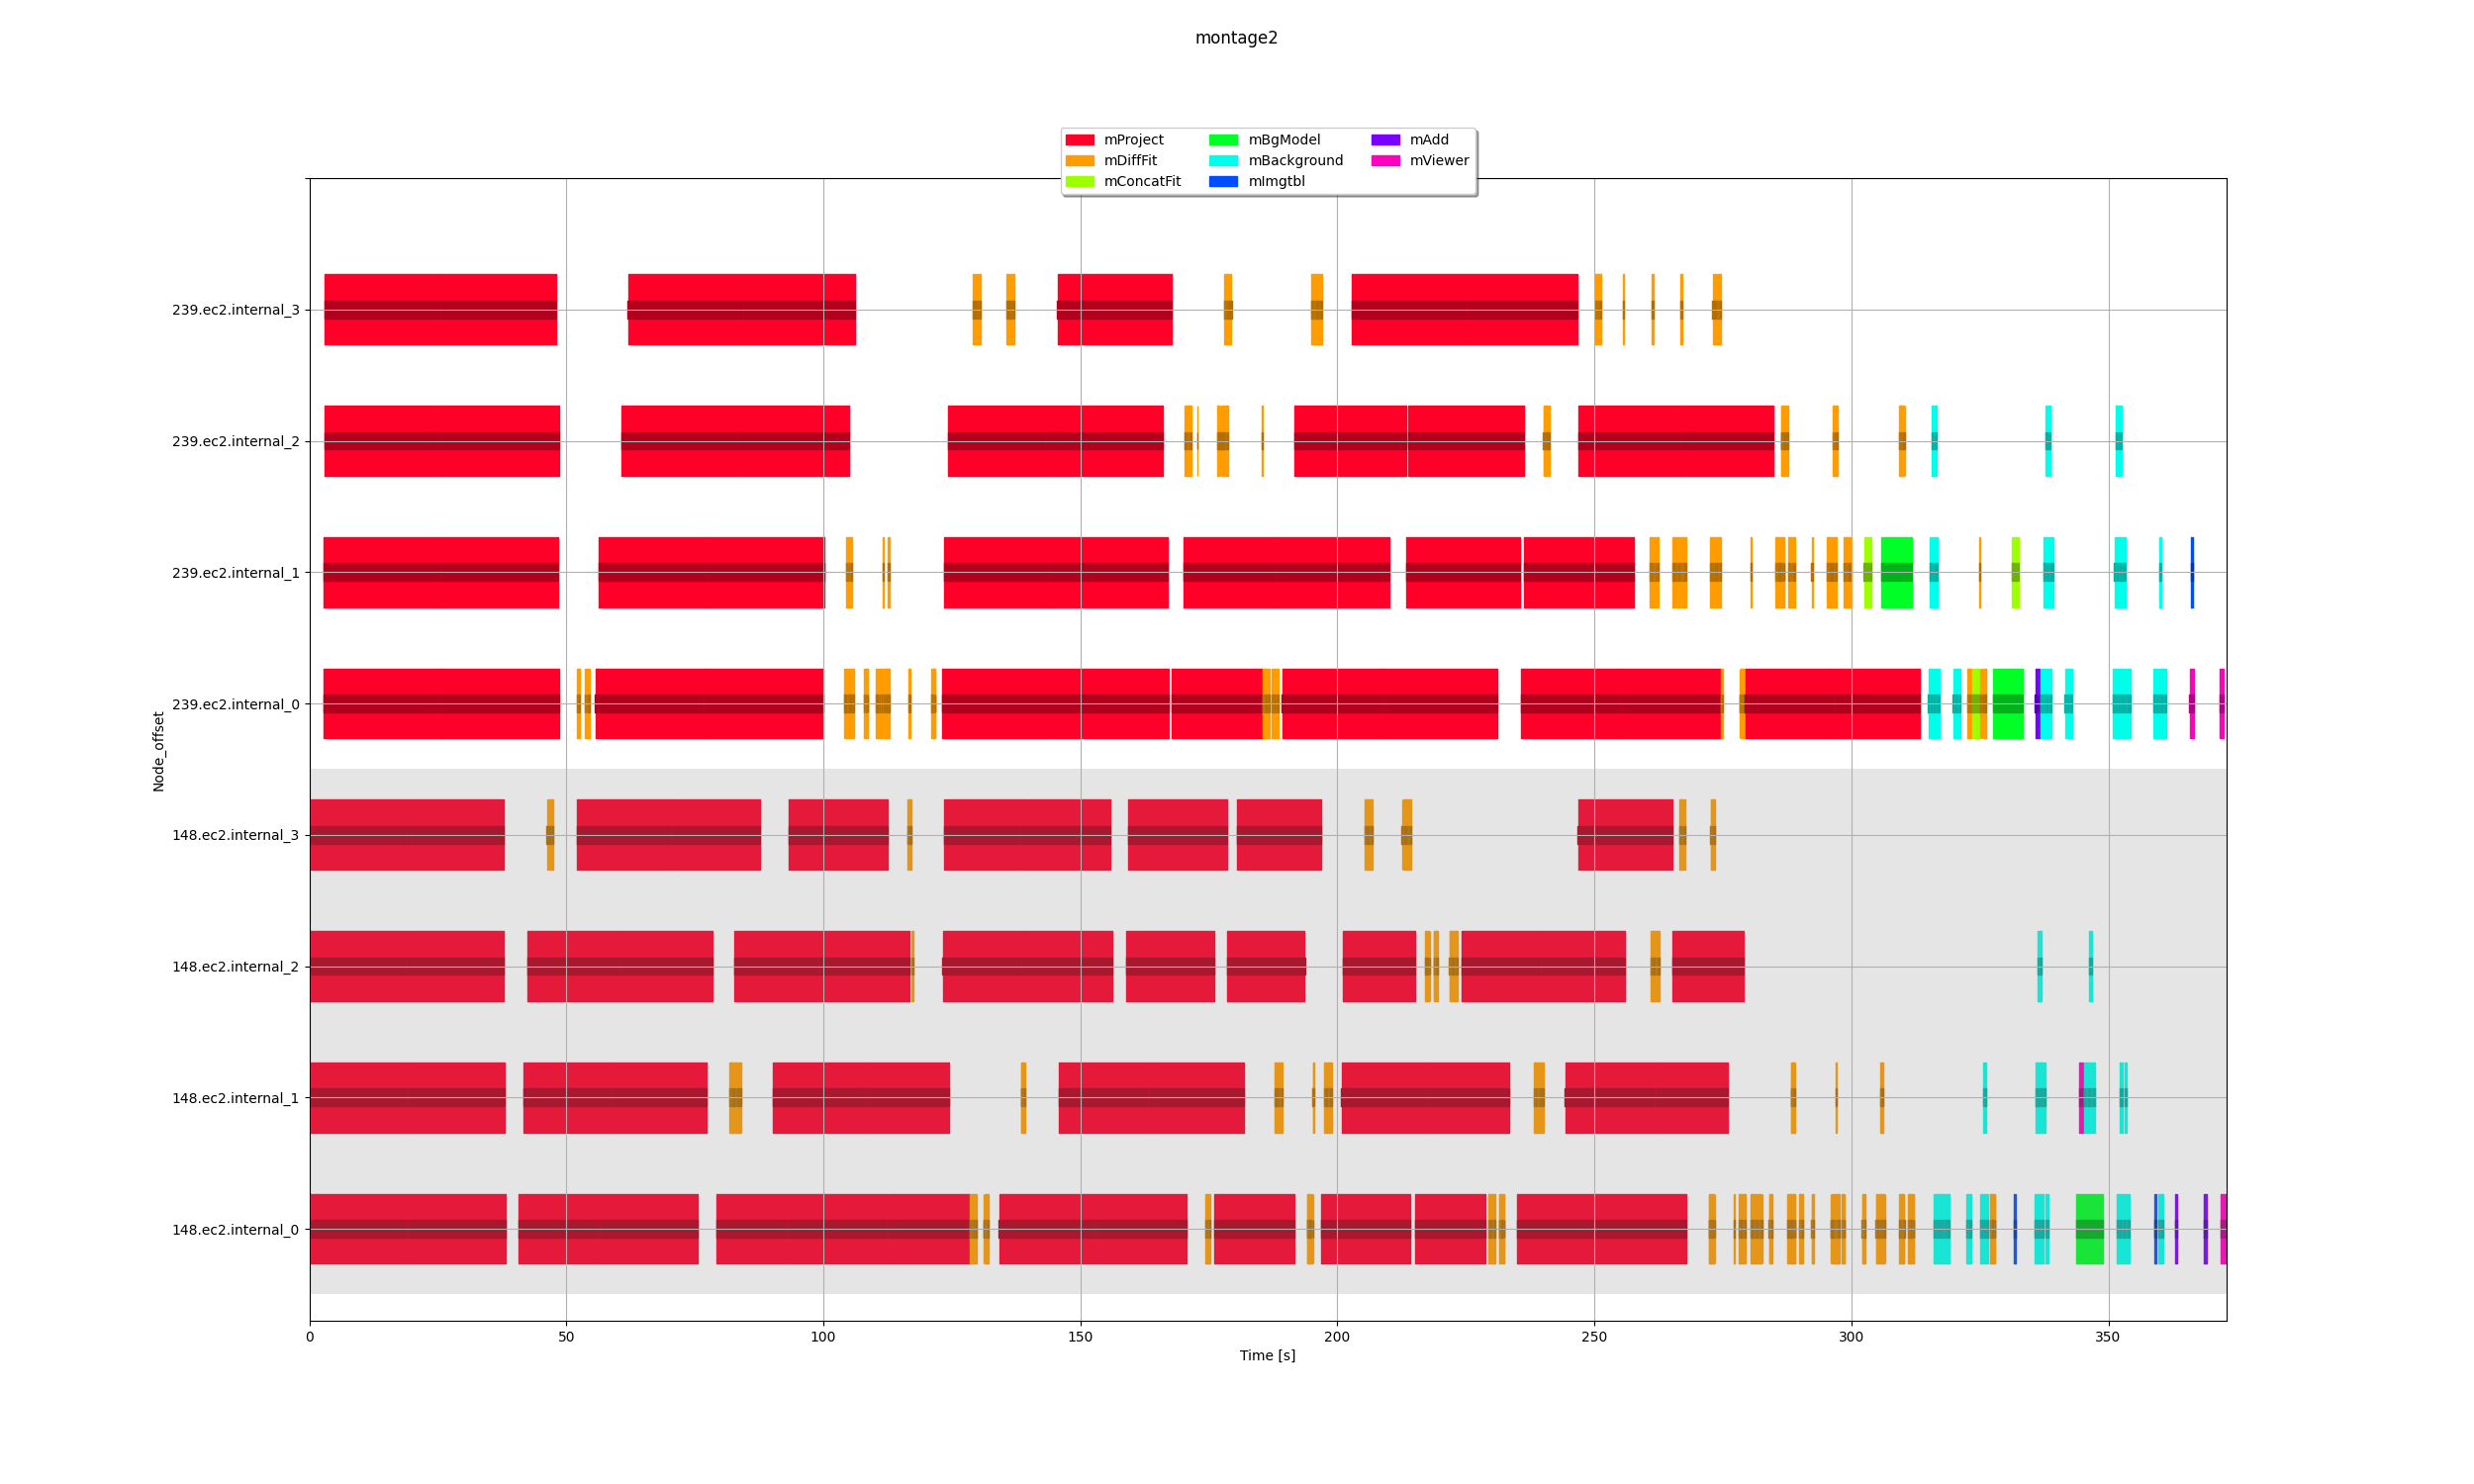
\includegraphics[width=1\linewidth]{figures/6-2-m0.25-agglo-empty.png}
\caption[Selected example execution trace for Montage2-v0.25 workflow with task clustering and no scheduler plugin]{w/o scheduler plugin}
\label{fig:evaluation:agglo:m025:empty}
\end{subfigure}
\begin{subfigure}{0.75\textwidth}
\centering
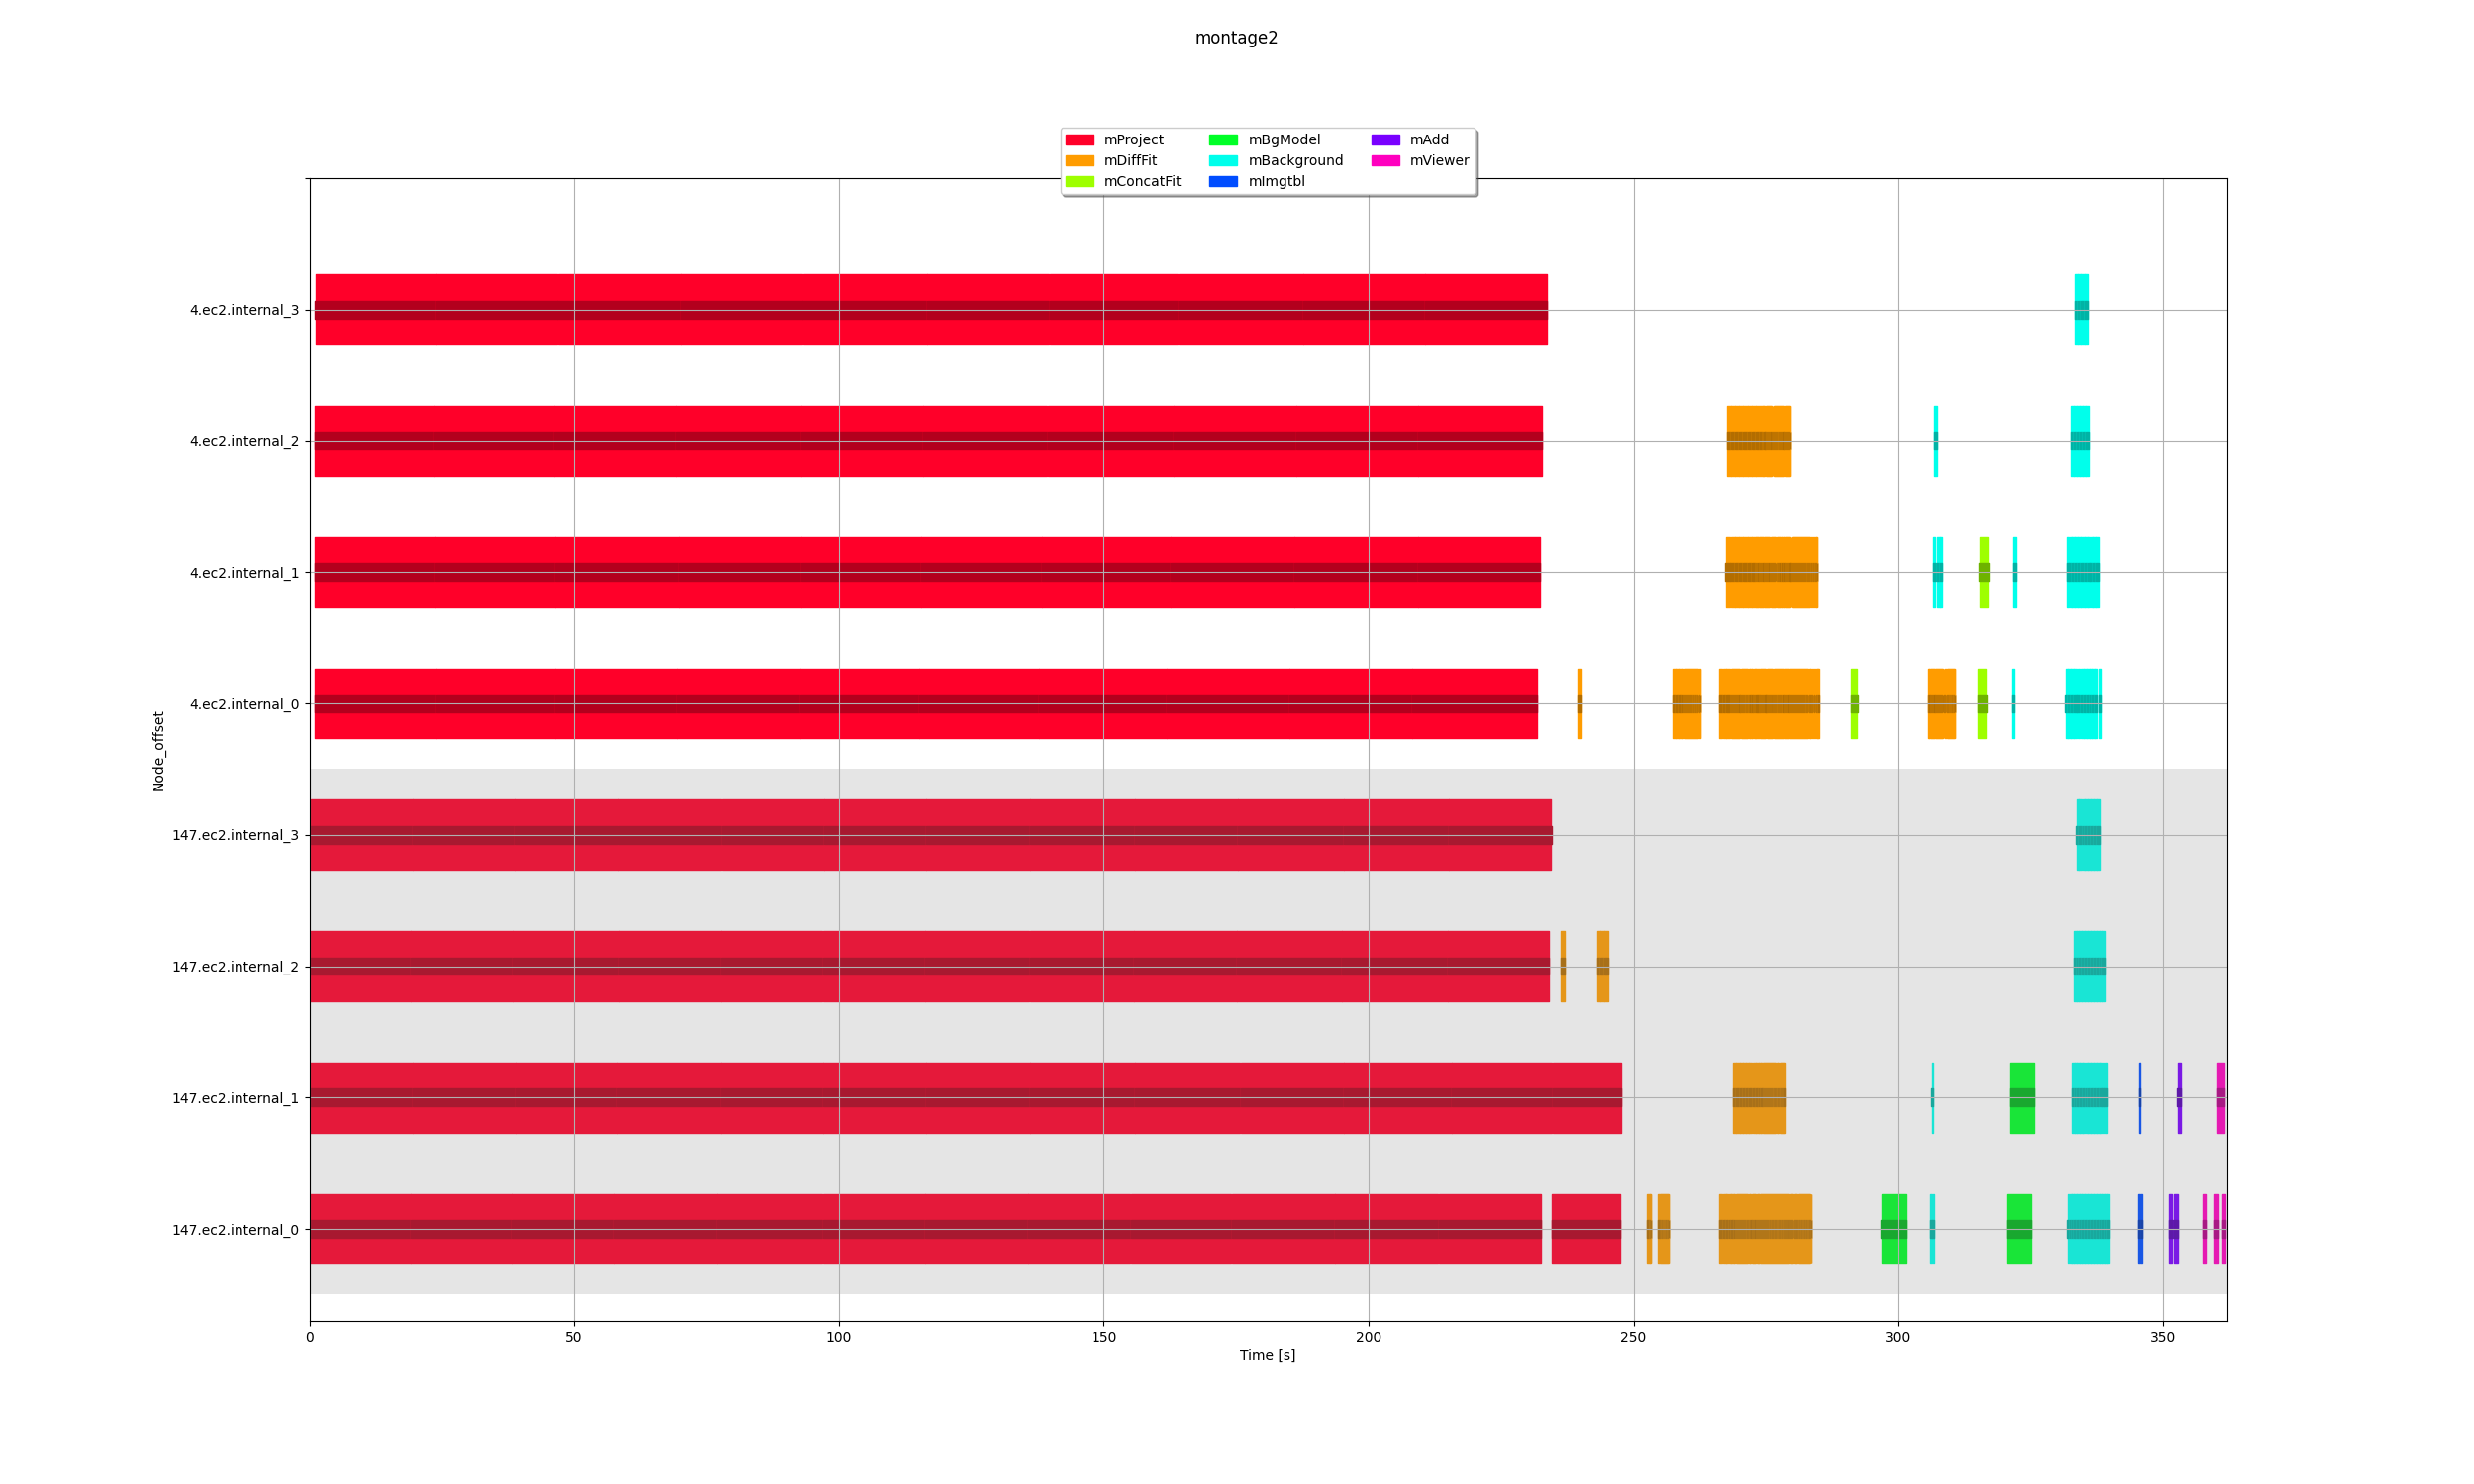
\includegraphics[width=1\linewidth]{figures/6-2-m0.25-agglo-heft.png}
\caption[Selected example execution traces for Montage2-v0.25 workflow with HEFT and task clustering]{HEFT}
\label{fig:evaluation:agglo:m025:heft}
\end{subfigure}
\begin{subfigure}{0.75\textwidth}
\centering
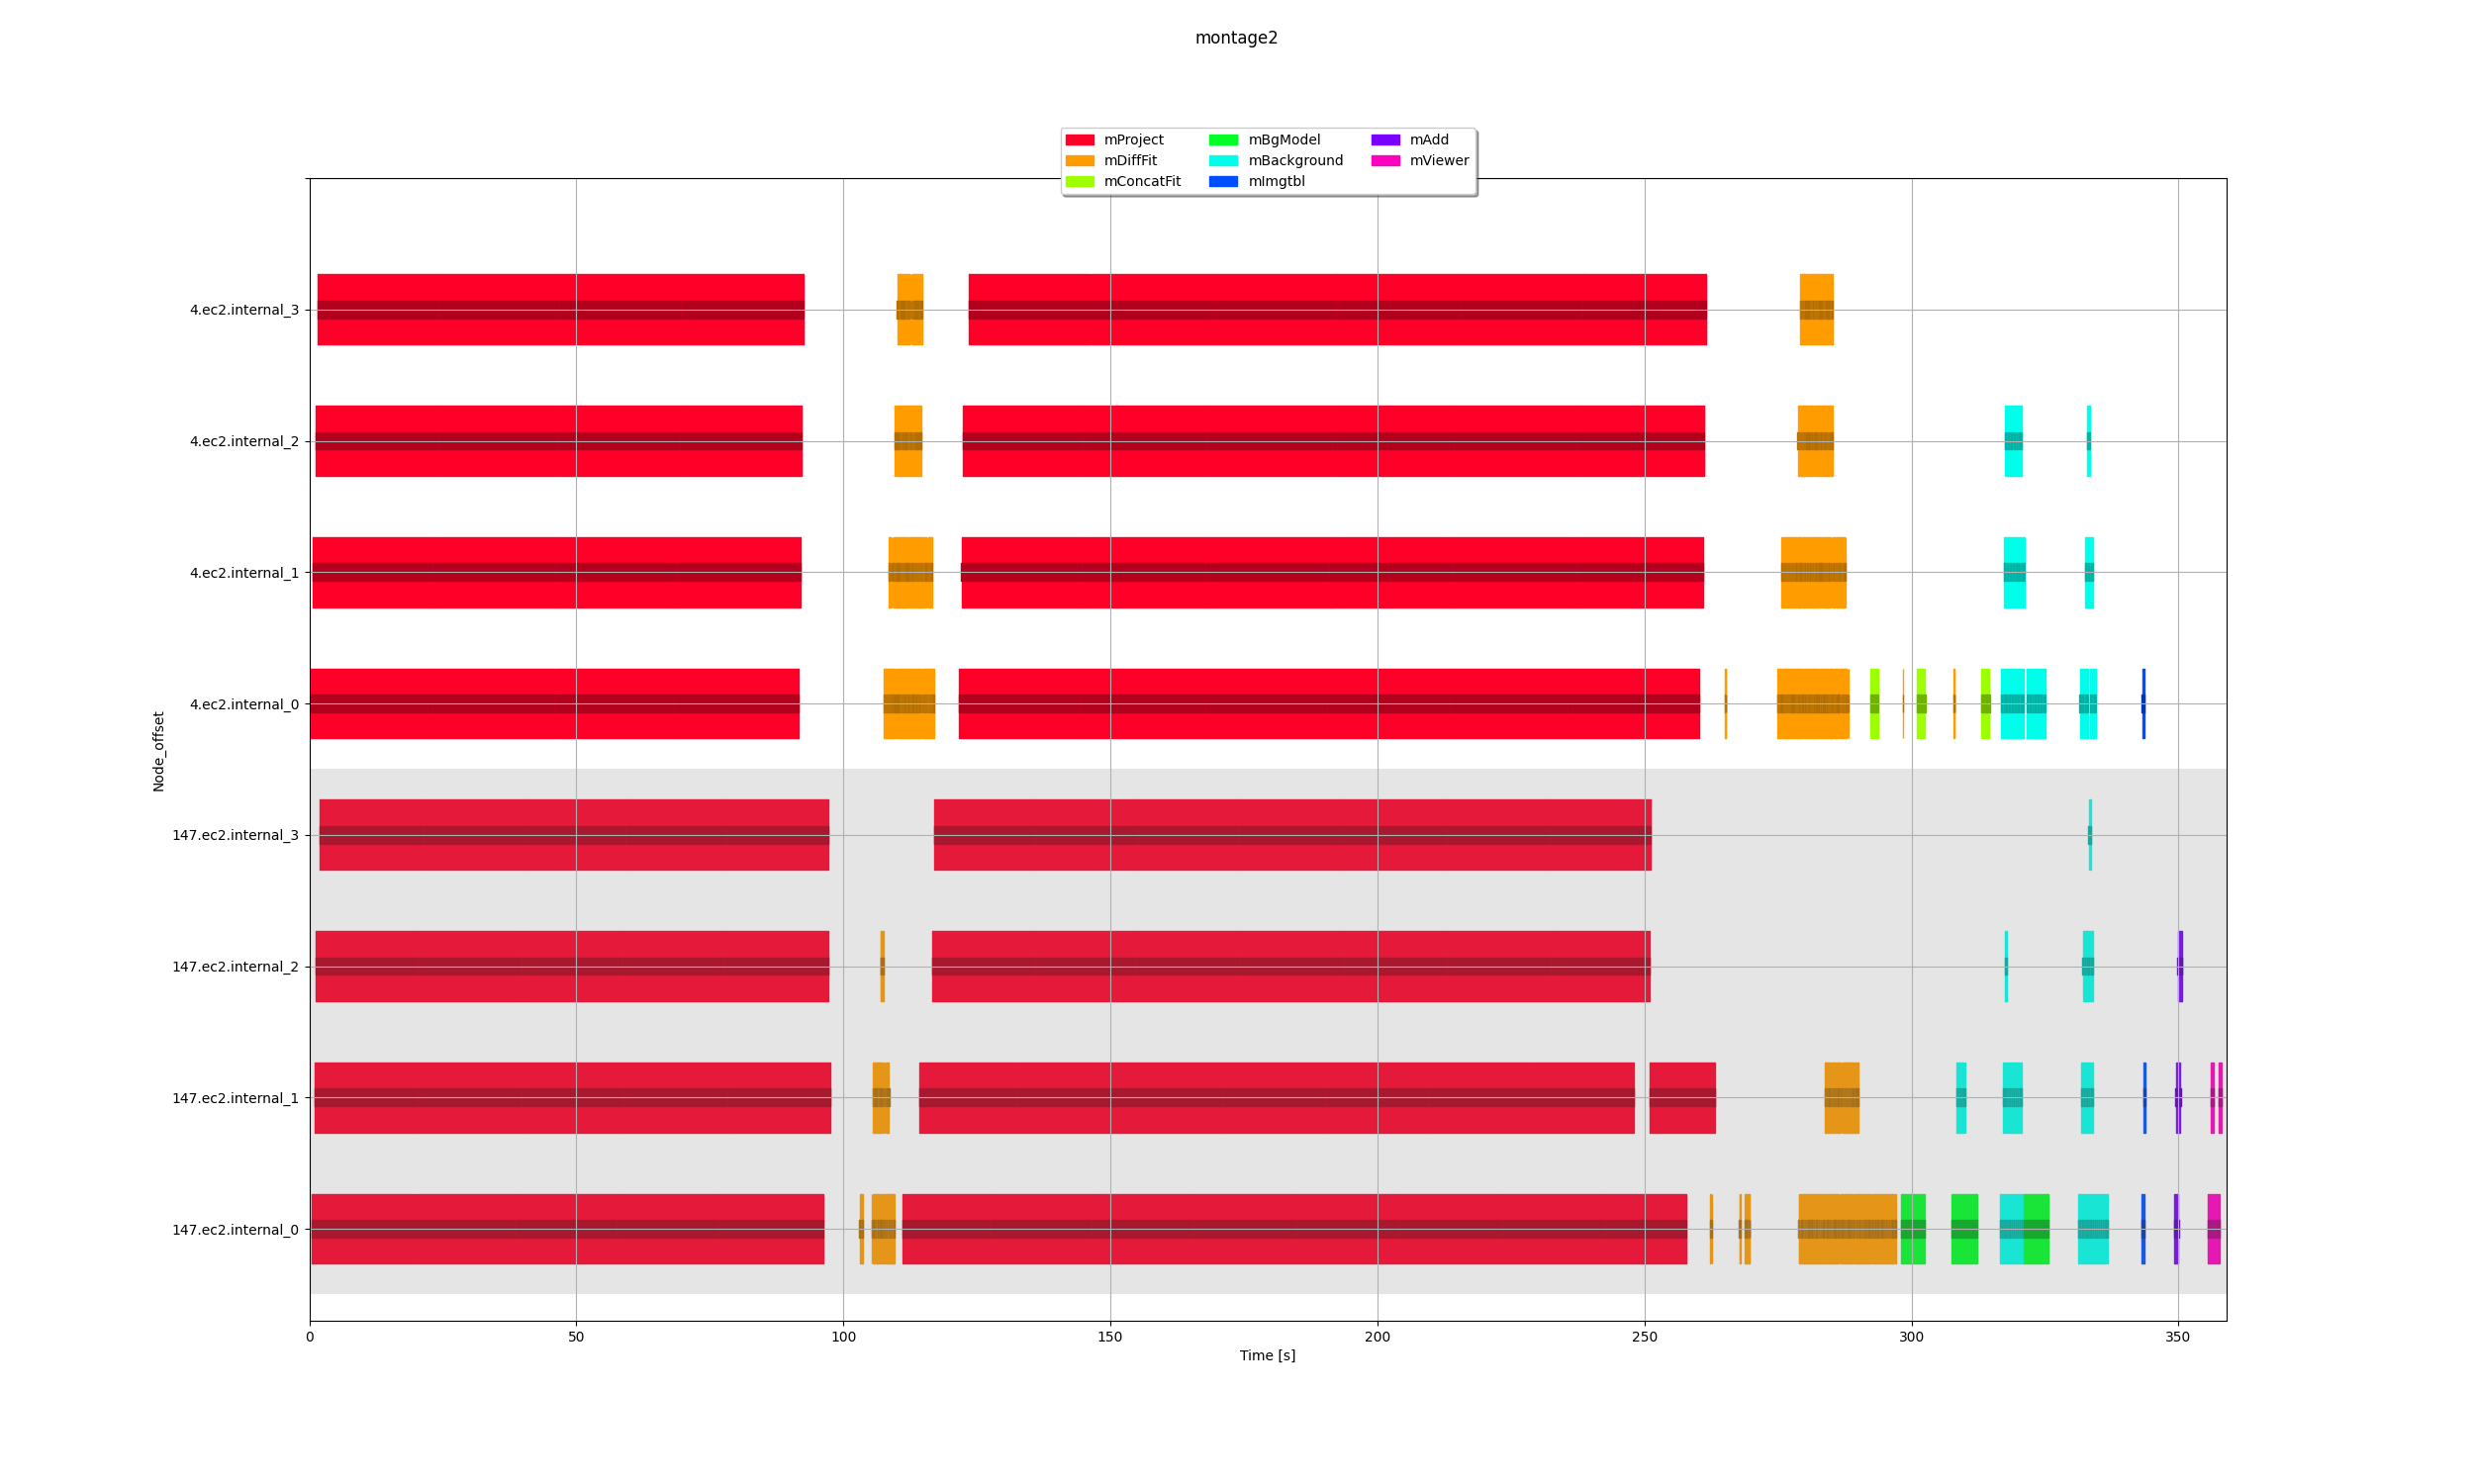
\includegraphics[width=1\linewidth]{figures/6-2-m0.25-agglo-peft.png}
\caption[Selected example execution traces for Montage2-v0.25 workflow with PEFT and task clustering]{PEFT}
\label{fig:evaluation:agglo:m025:peft}
\end{subfigure}
\centering
%%
\caption[Selected example execution traces for Montage2-v0.25 workflow with task clustering]{Selected example execution traces for Montage2-v0.25 workflow with task clustering.}
\label{fig:evaluation:agglo:m025:plugin}
\end{figure}
%%%% KONIEC FIG @@@@@@@@@@@


The two-step scheduling seems to work better for larger workflows as well.
In the case of Montage2-v1.0 workflow, both HEFT and PEFT schedules have proven to be more effective than the default solution, with HEFT shortening the makespan by roughly 8\% and reducing CO by over 80\%, according to the metric values (\cref{tab:metrics-clustering-m10}).
Unexpectedly, the achieved job slowdown for approaches with applied static scheduling is for the first time better than the others.


%%% Tabelka z metrykami - Montage-1.0
\begin{table}[H]
    \centering
    \begin{tabular}{|c|c|c|c|c|}
    \cline{1-5}
        \multirow{2}{*}{Approach} 
        &
        \multicolumn{4}{|c|}{Metrics} \\
    \cline{2-5}
        & Makespan & Job slowdown & SLR & CO \\
    \cline{1-5}
        kube-scheduler & 779 & 537 & 7.6 & 8200 \\
    \cline{1-5}
        HEFT + kube-scheduler & 712 & 239 & 7.1 & 1271 \\
    \cline{1-5}
        PEFT + kube-scheduler & 770 & 256 & 7.3 & 2008 \\
    \cline{1-5}
    \end{tabular}
    \caption{Average metric results of Montage2-v1.0 execution with task clustering}
    \label{tab:metrics-clustering-m10}
\end{table}
%%%

There is no much difference in an execution flow between larger and smaller Montage workflows.
From the \cref{fig:evaluation:agglo:m10:plugin}, it seems that all analyzed approaches follow the already observed behaviour.

Looking at the results, running a lower number of containers, but with a longer lifespan, has been proven to positively impact the overall workflow execution performance, no matter which application is run.
The other valuable conclusion of the provided analysis is that larger workflows have their possible makespan reduction highly reliant on lowering container overhead times, while the smaller ones are slightly more schedule sensitive.

Lastly, it is worth mentioning that with task clustering, the problem of low workload parallelization, observed during the experiment without agglomeration, has been resolved.
Grouping tasks into containerized jobs prolongs the container lifespan, which makes it easier to distribute the load across the node resources in a Kubernetes cluster.


%%%%%% Traces - Montage-v1.0
\begin{figure}[H]
\begin{subfigure}{0.75\textwidth}
\centering
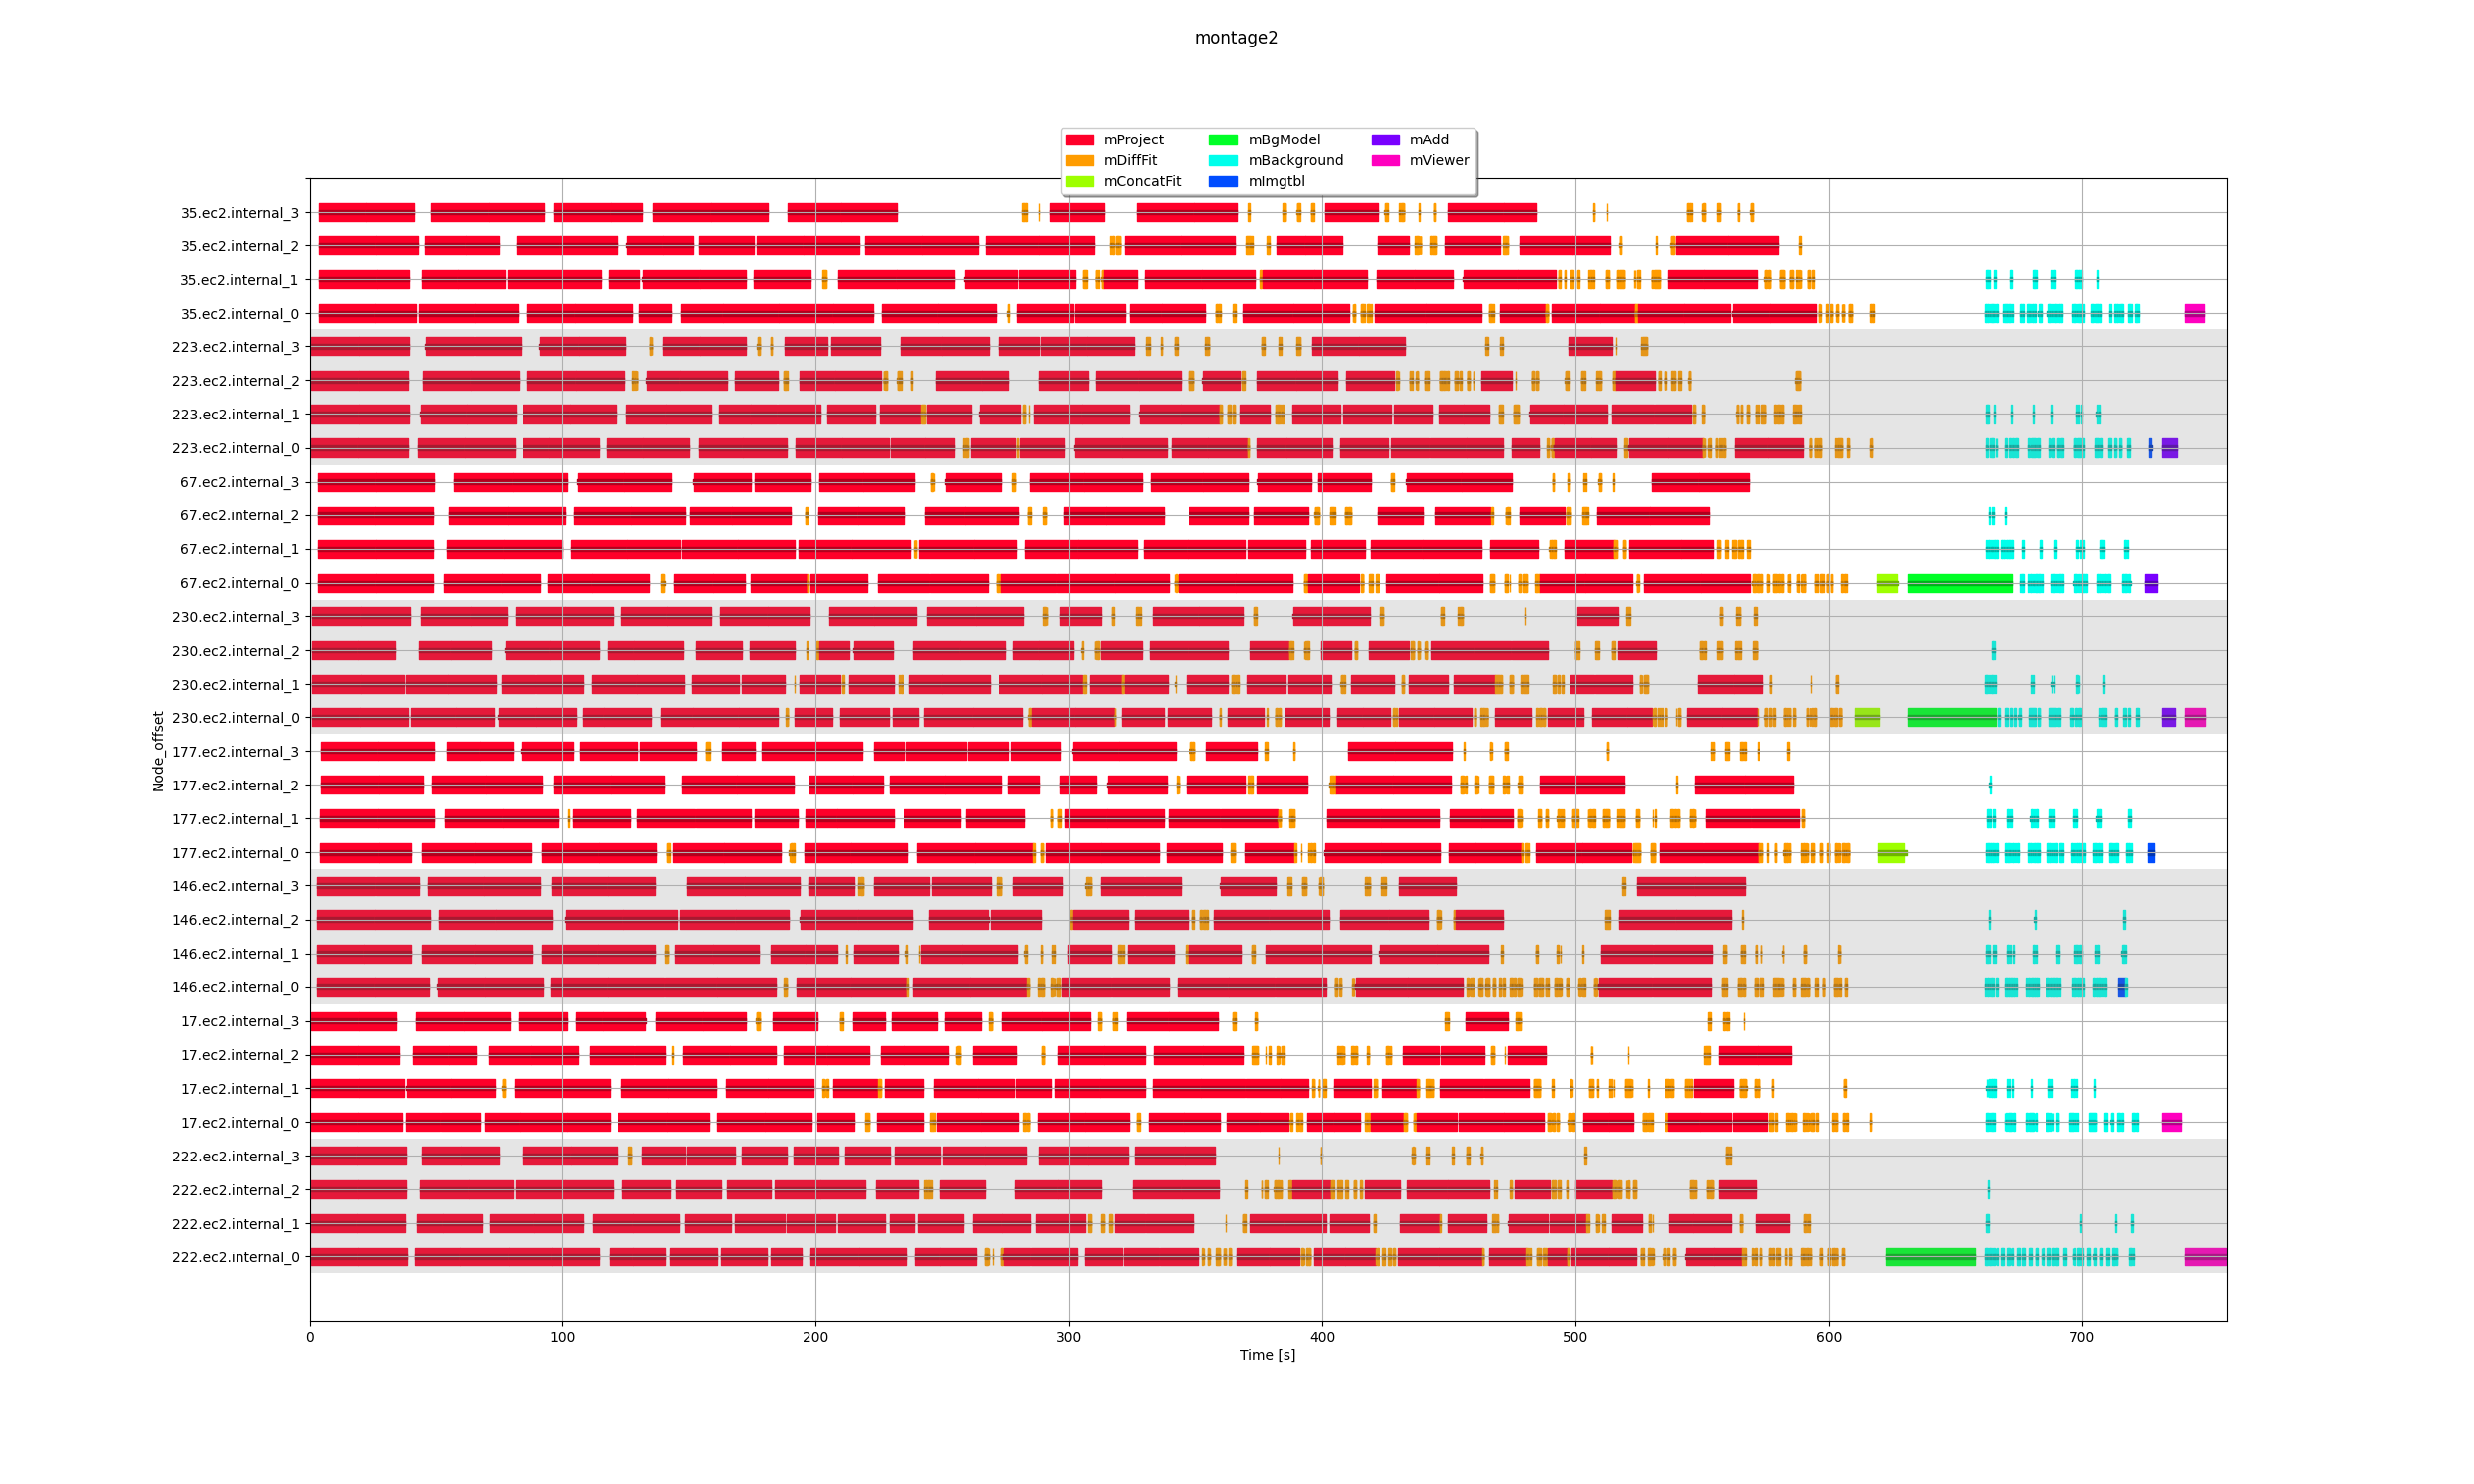
\includegraphics[width=1\linewidth]{figures/6-2-m1.0-agglo-empty.png}
\caption[Selected example execution trace for Montage2-v1.0 workflow with task clustering and no scheduler plugin]{w/o scheduler plugin}
\label{fig:evaluation:agglo:m10:empty}
\end{subfigure}
\begin{subfigure}{0.75\textwidth}
\centering
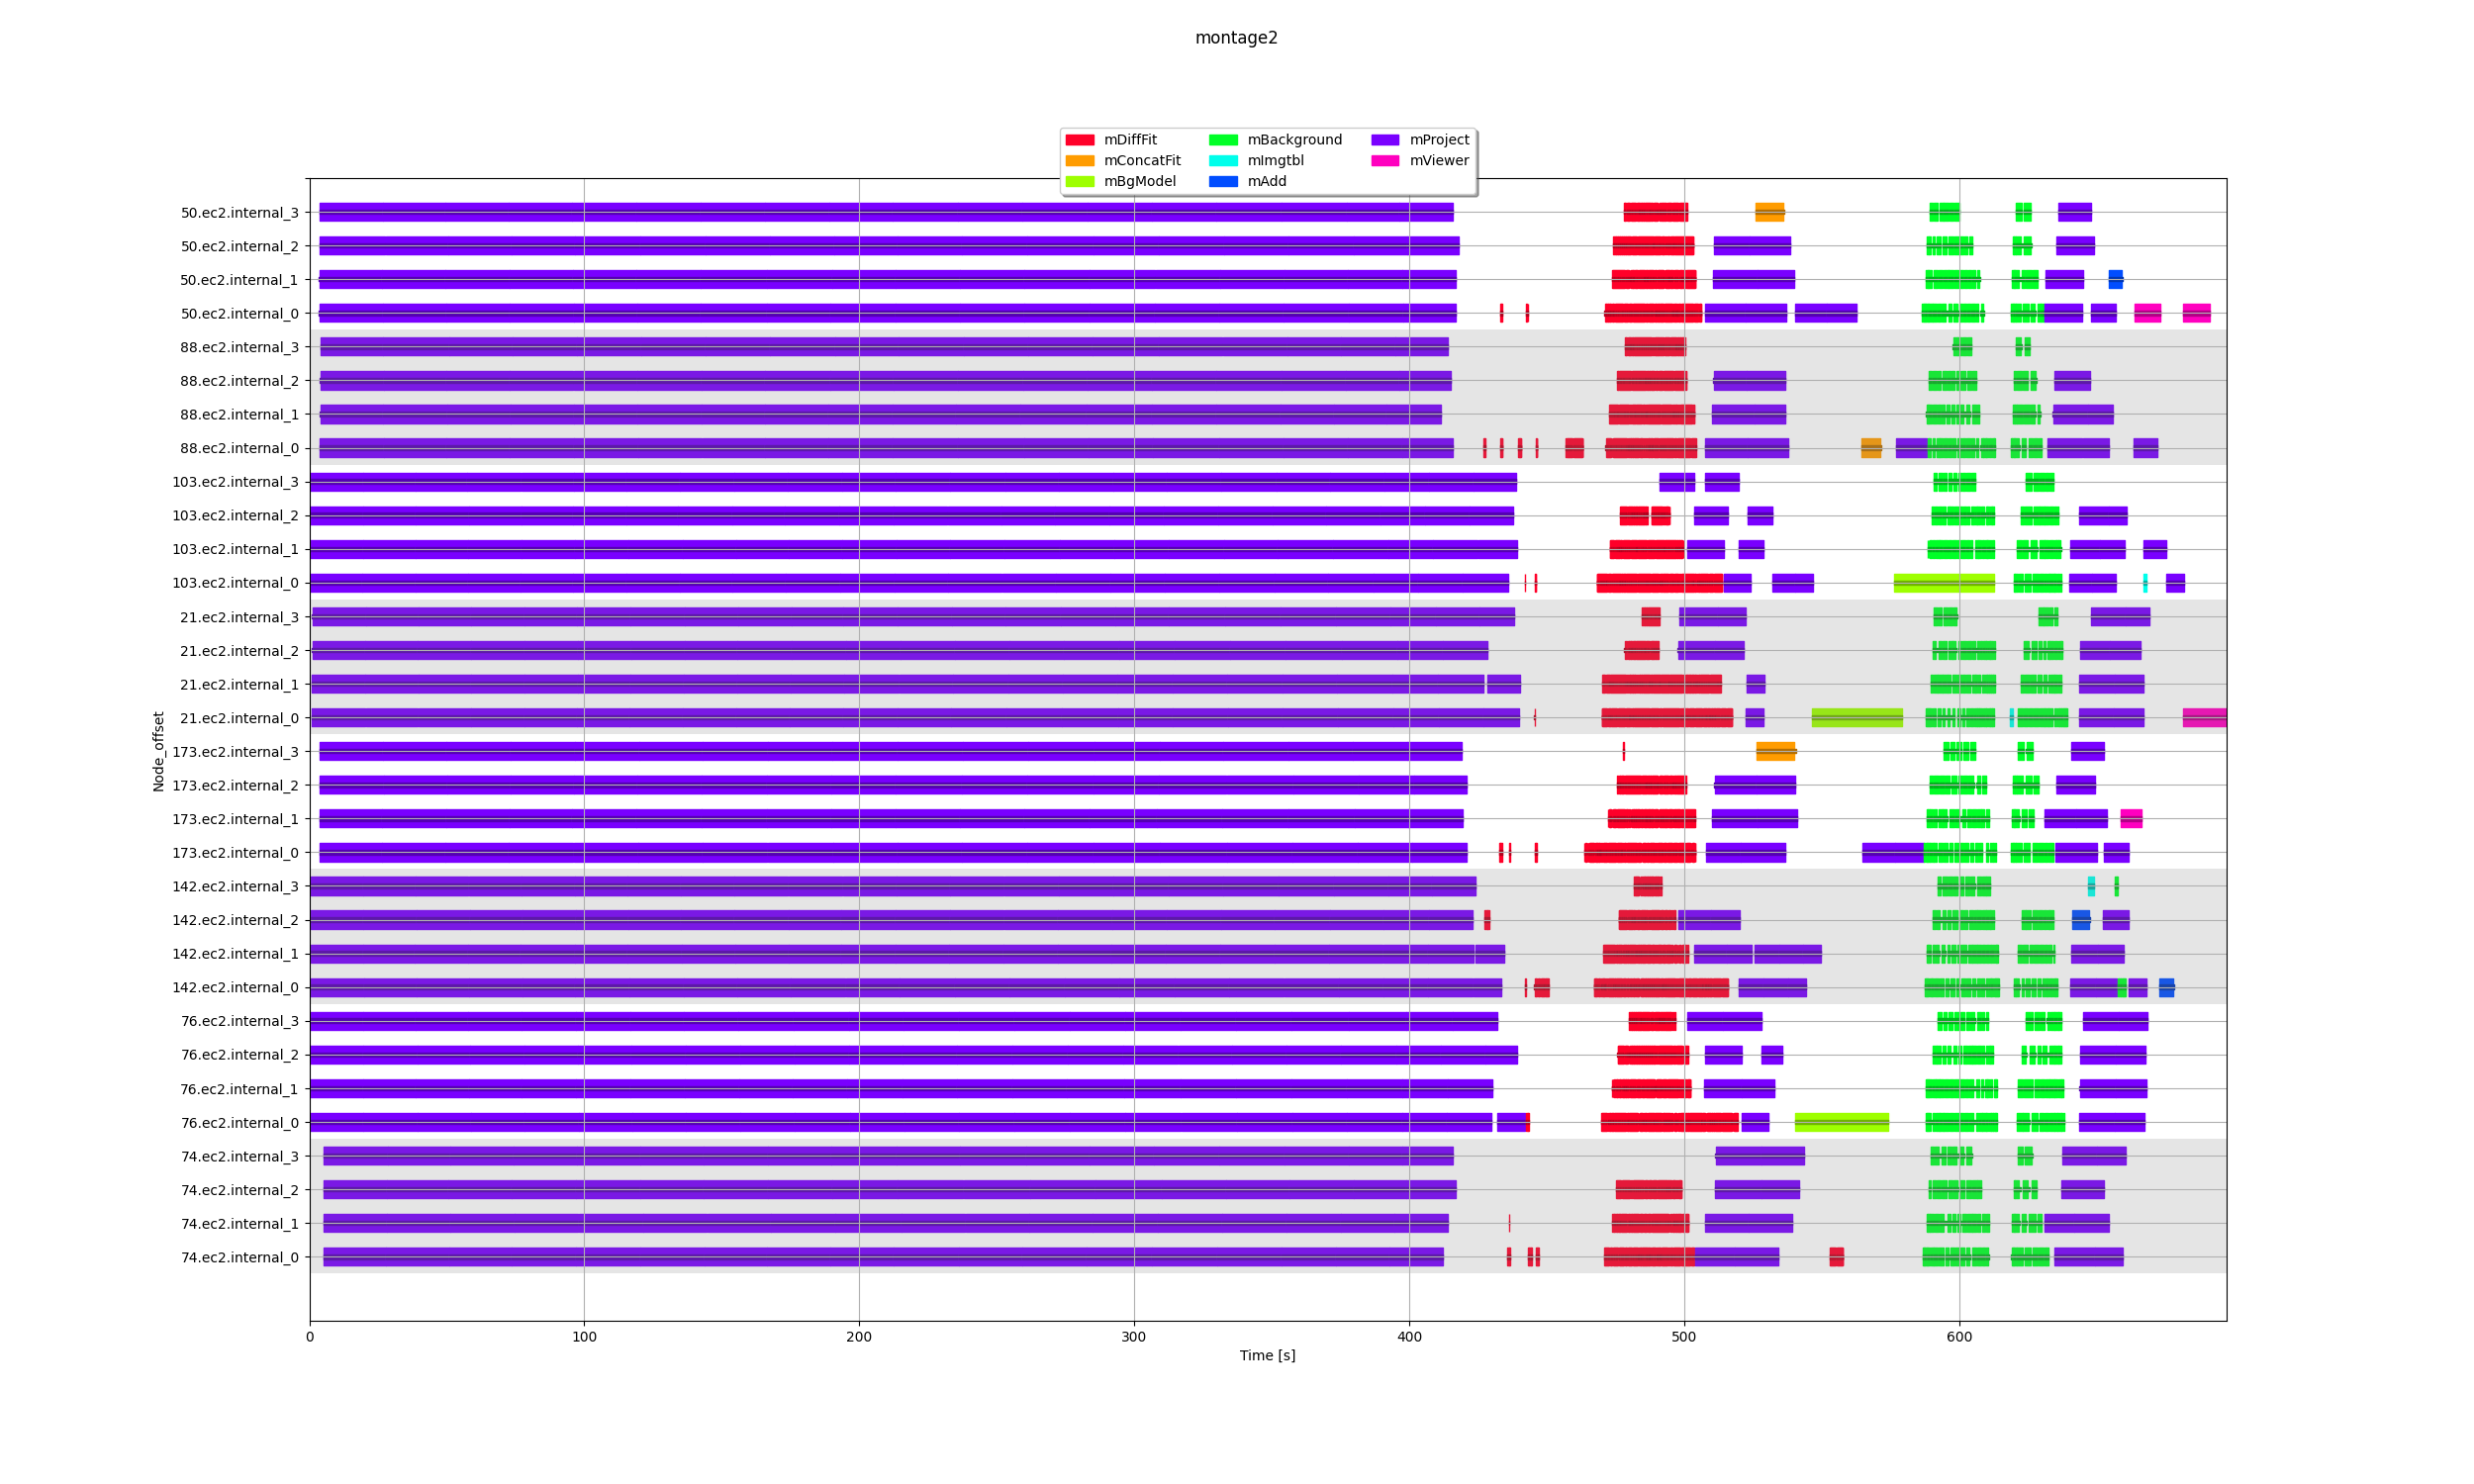
\includegraphics[width=1\linewidth]{figures/6-2-m1.0-agglo-heft.png}
\caption[Selected example execution traces for Montage2-v1.0 workflow with HEFT and task clustering]{HEFT}
\label{fig:evaluation:agglo:m10:heft}
\end{subfigure}
\begin{subfigure}{0.75\textwidth}
\centering
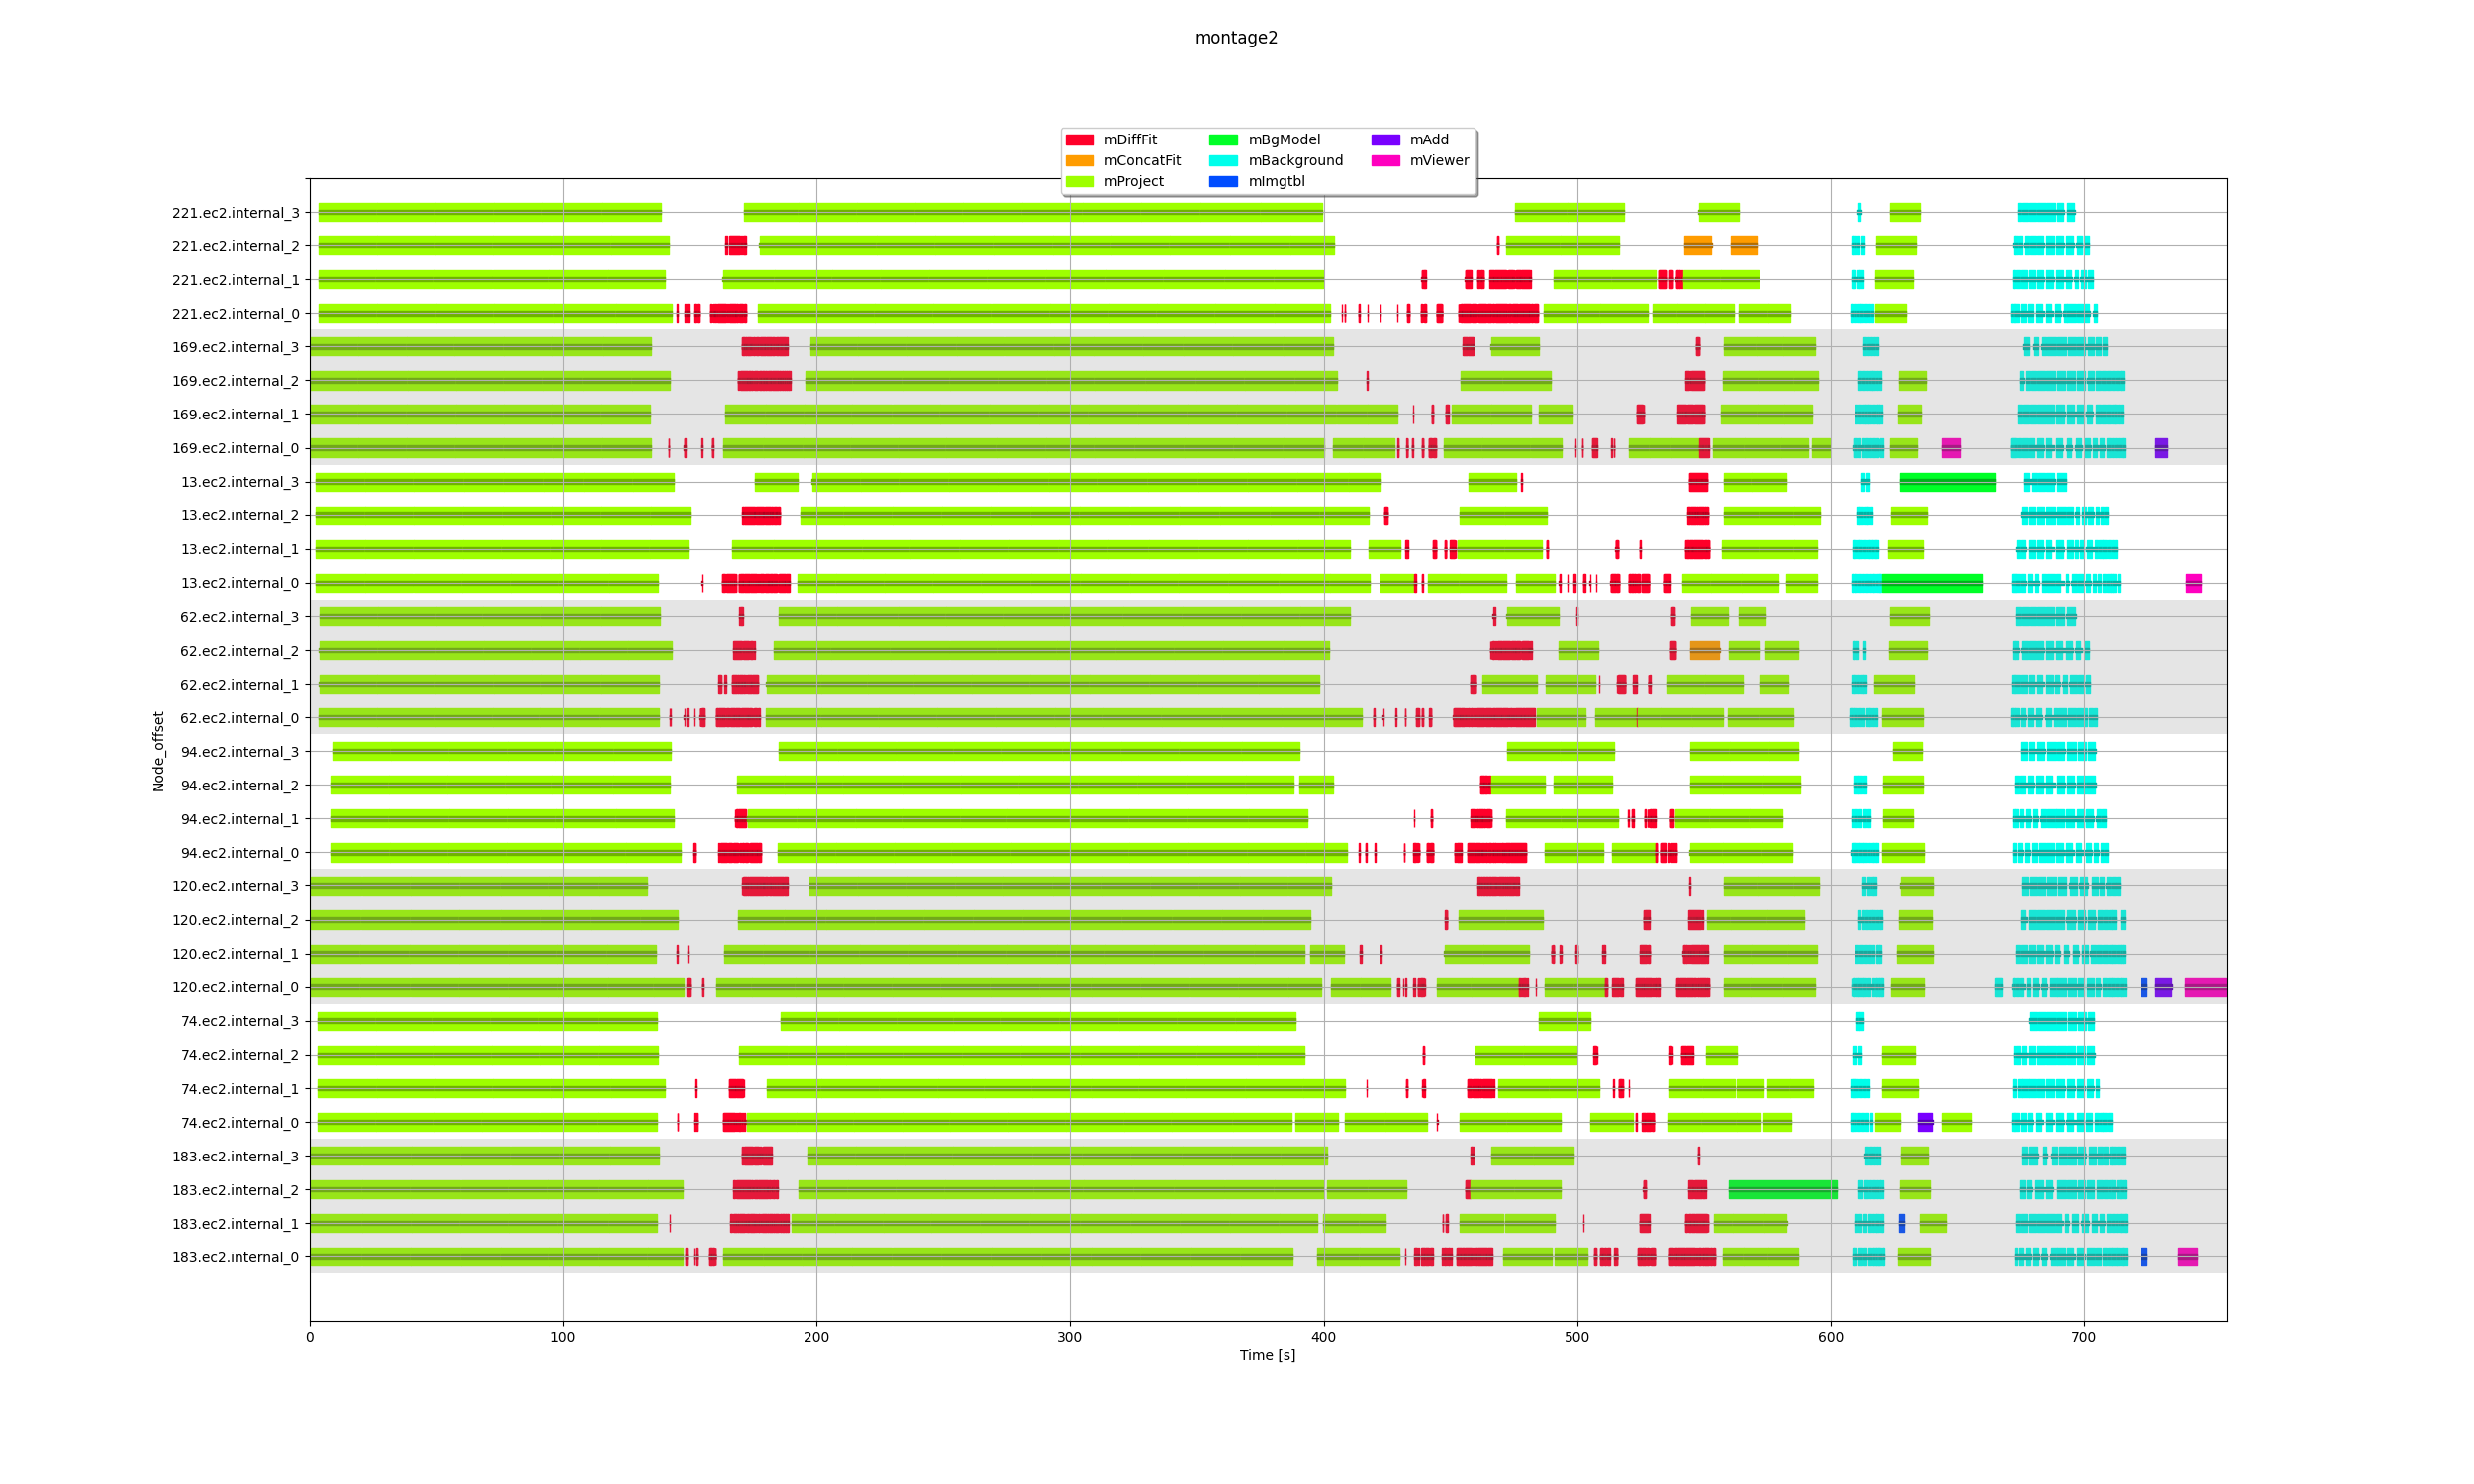
\includegraphics[width=1\linewidth]{figures/6-2-m1.0-agglo-peft.png}
\caption[Selected example execution traces for Montage2-v1.0 workflow with PEFT and task clustering]{PEFT}
\label{fig:evaluation:agglo:m10:peft}
\end{subfigure}
\centering
%%
\caption[Selected example execution traces for Montage2-v1.0 workflow with task clustering]{Selected example execution traces for Montage2-v1.0 workflow with task clustering.}
\label{fig:evaluation:agglo:m10:plugin}
\end{figure}
%%%%%% 


%%%%
% \begin{figure}[H]
% \centering
% 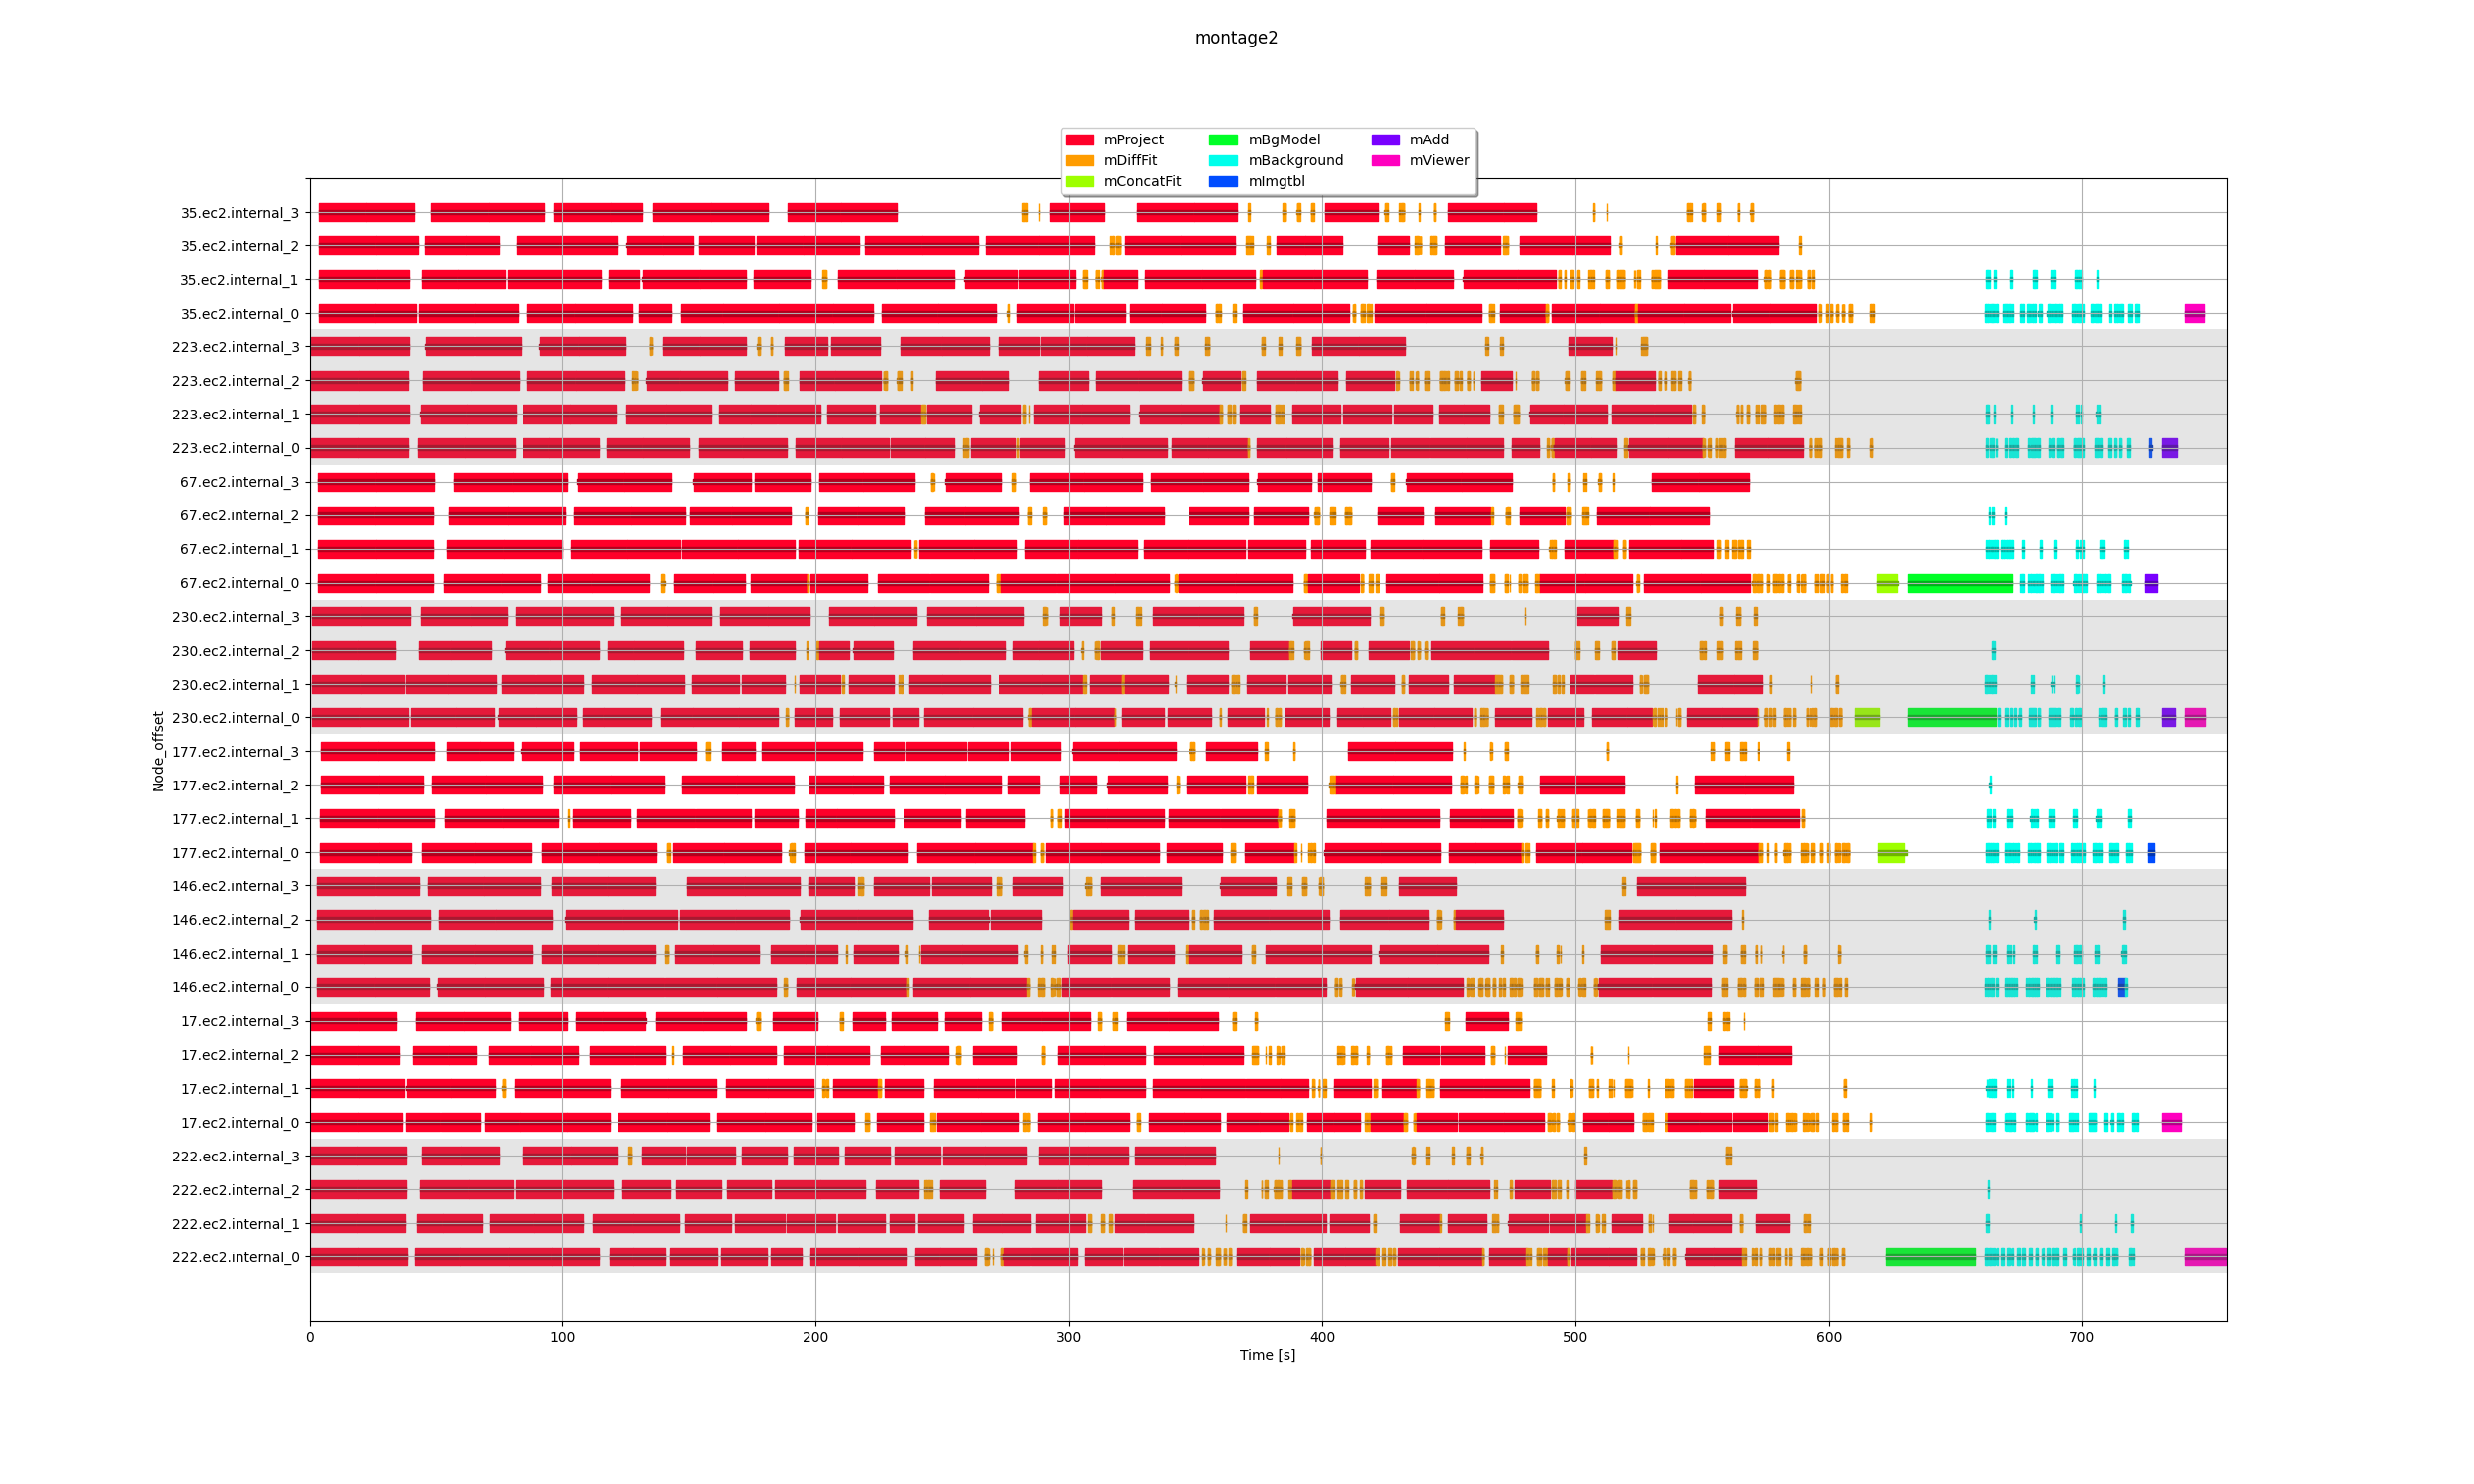
\includegraphics[width=1\linewidth]{figures/6-2-m1.0-agglo-empty.png}
% \caption[Task clustering without workflow scheduling - Montage-1.0]{Task clustering without workflow scheduling - Montage-1.0.}
% \label{fig:evaluation:agglo:m10:empty}
% \end{figure}

% \begin{figure}[H]
% \centering
% 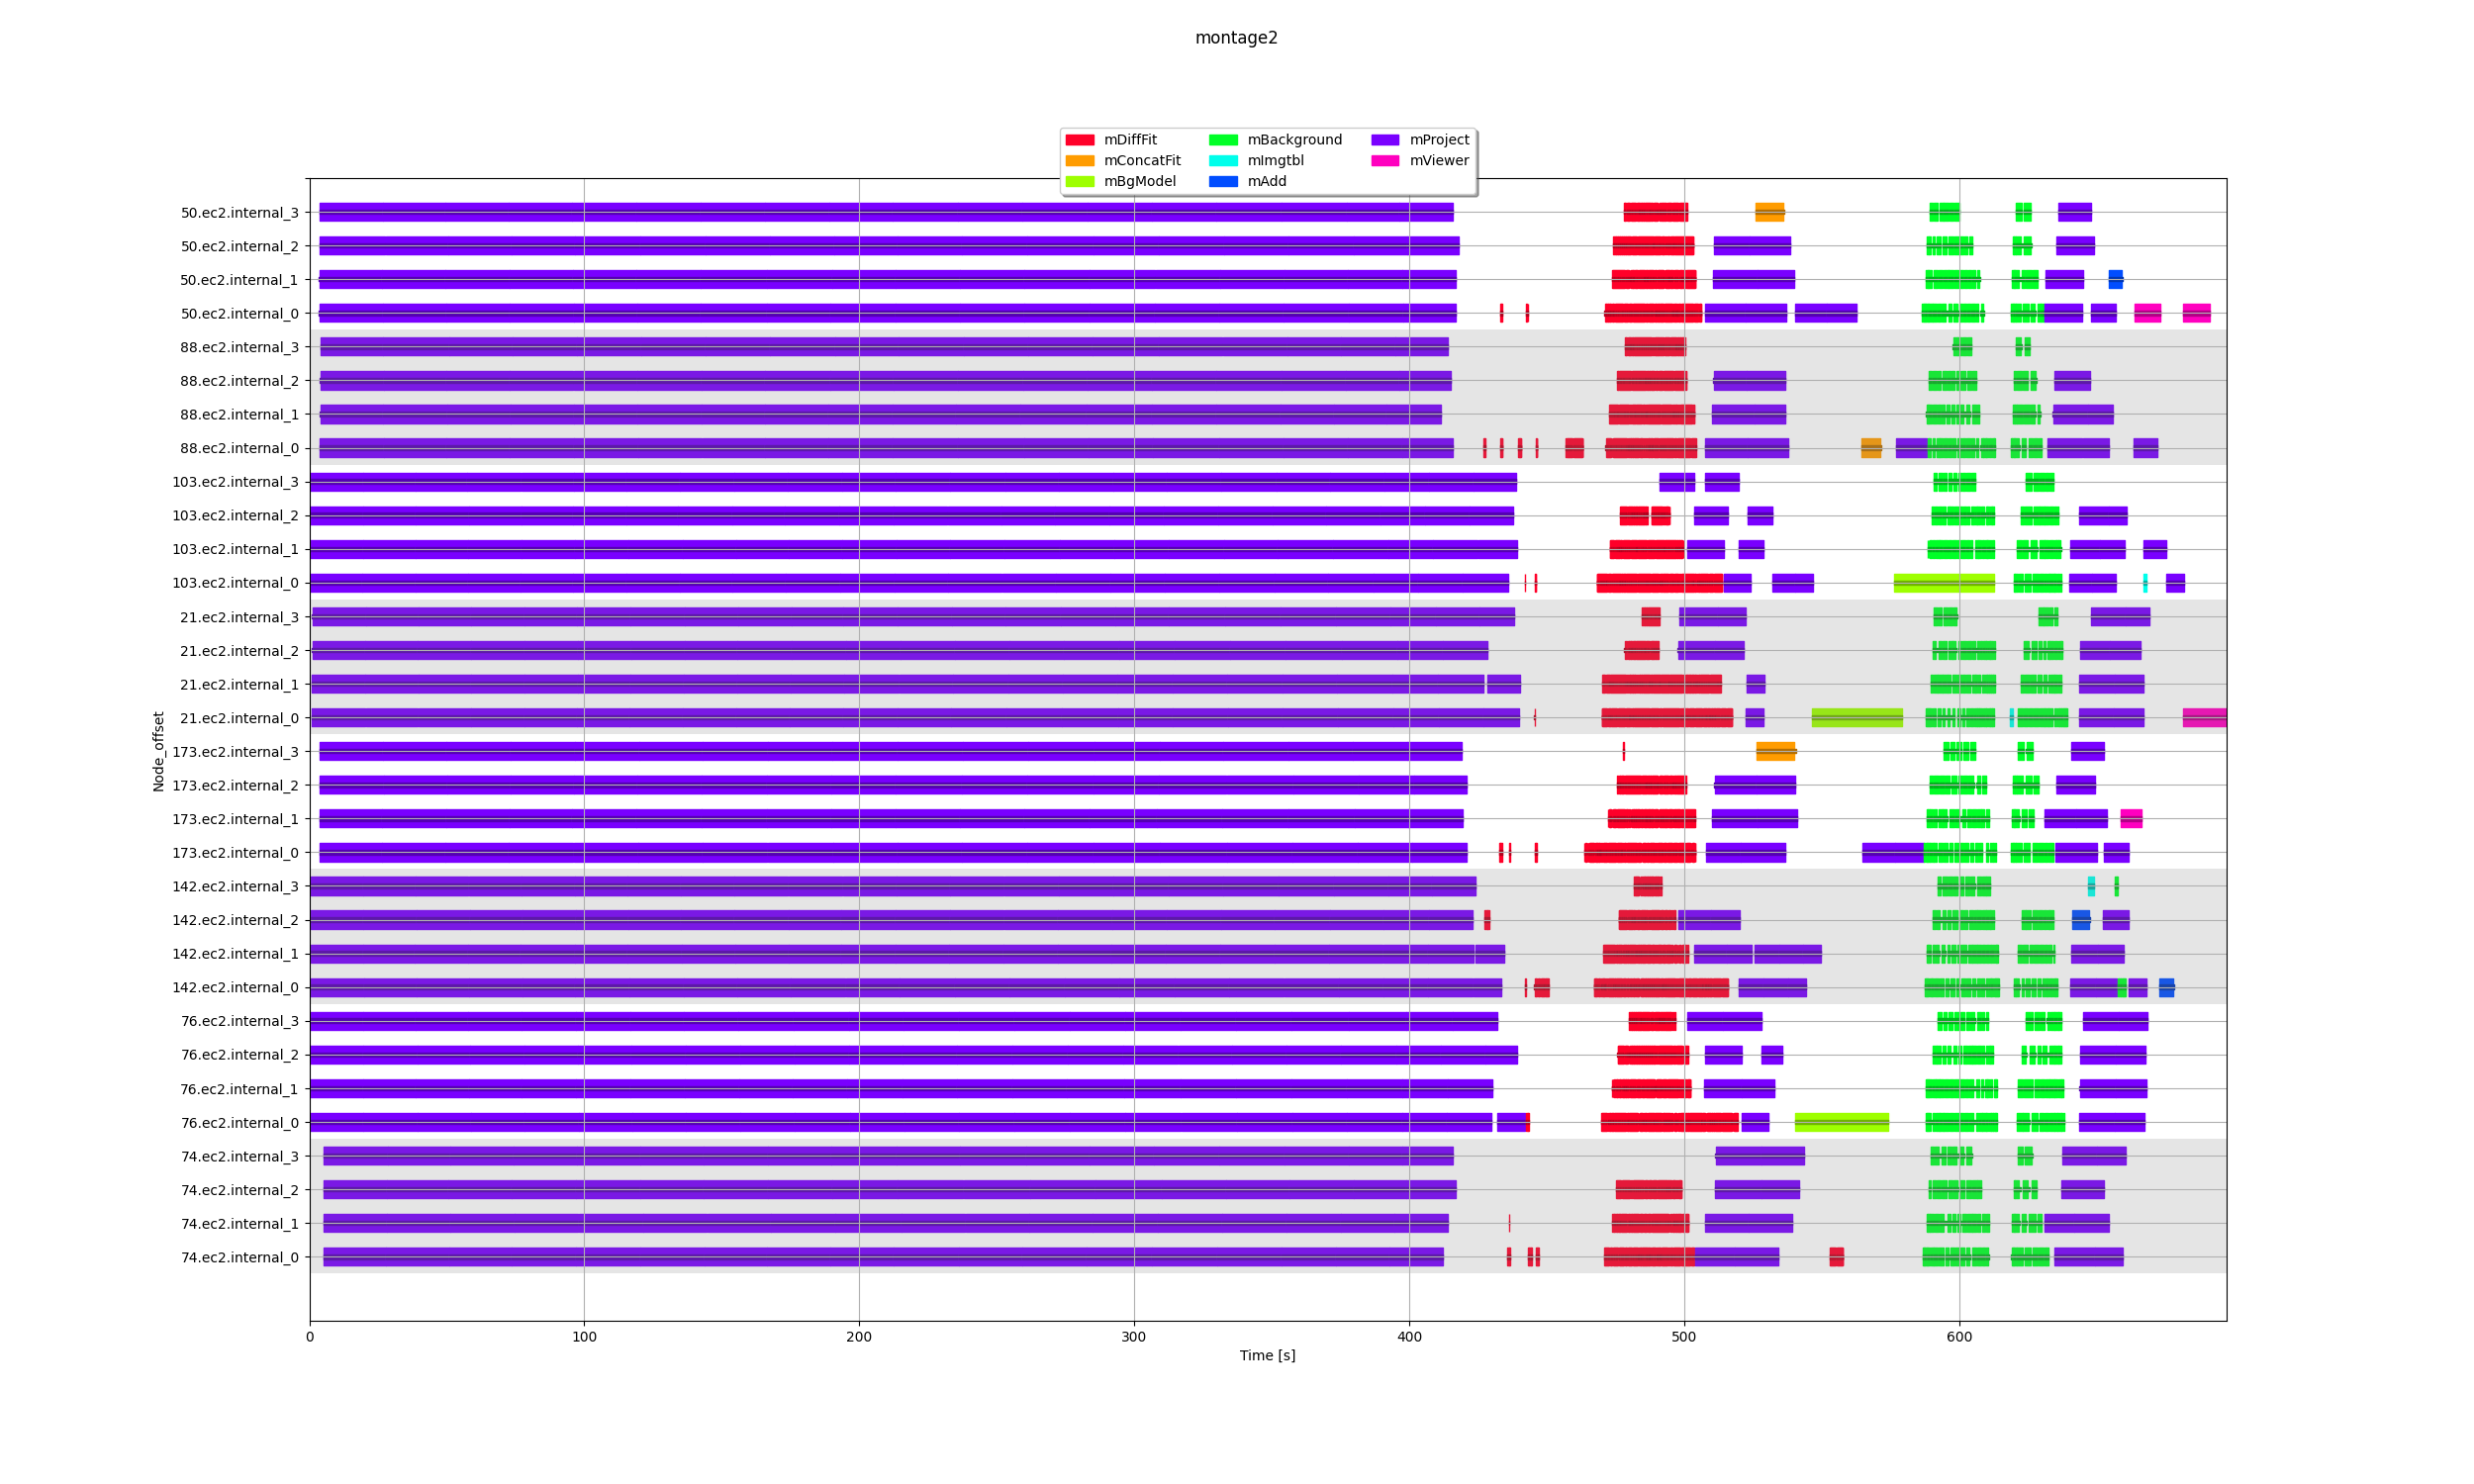
\includegraphics[width=1\linewidth]{figures/6-2-m1.0-agglo-heft.png}
% \caption[Task clustering on HEFT-planned schedule - Montage-1.0]{Task clustering on HEFT-planned schedule - Montage-0.25.}
% \label{fig:evaluation:agglo:m10:heft}
% \end{figure}

% \begin{figure}[H]
% \centering
% 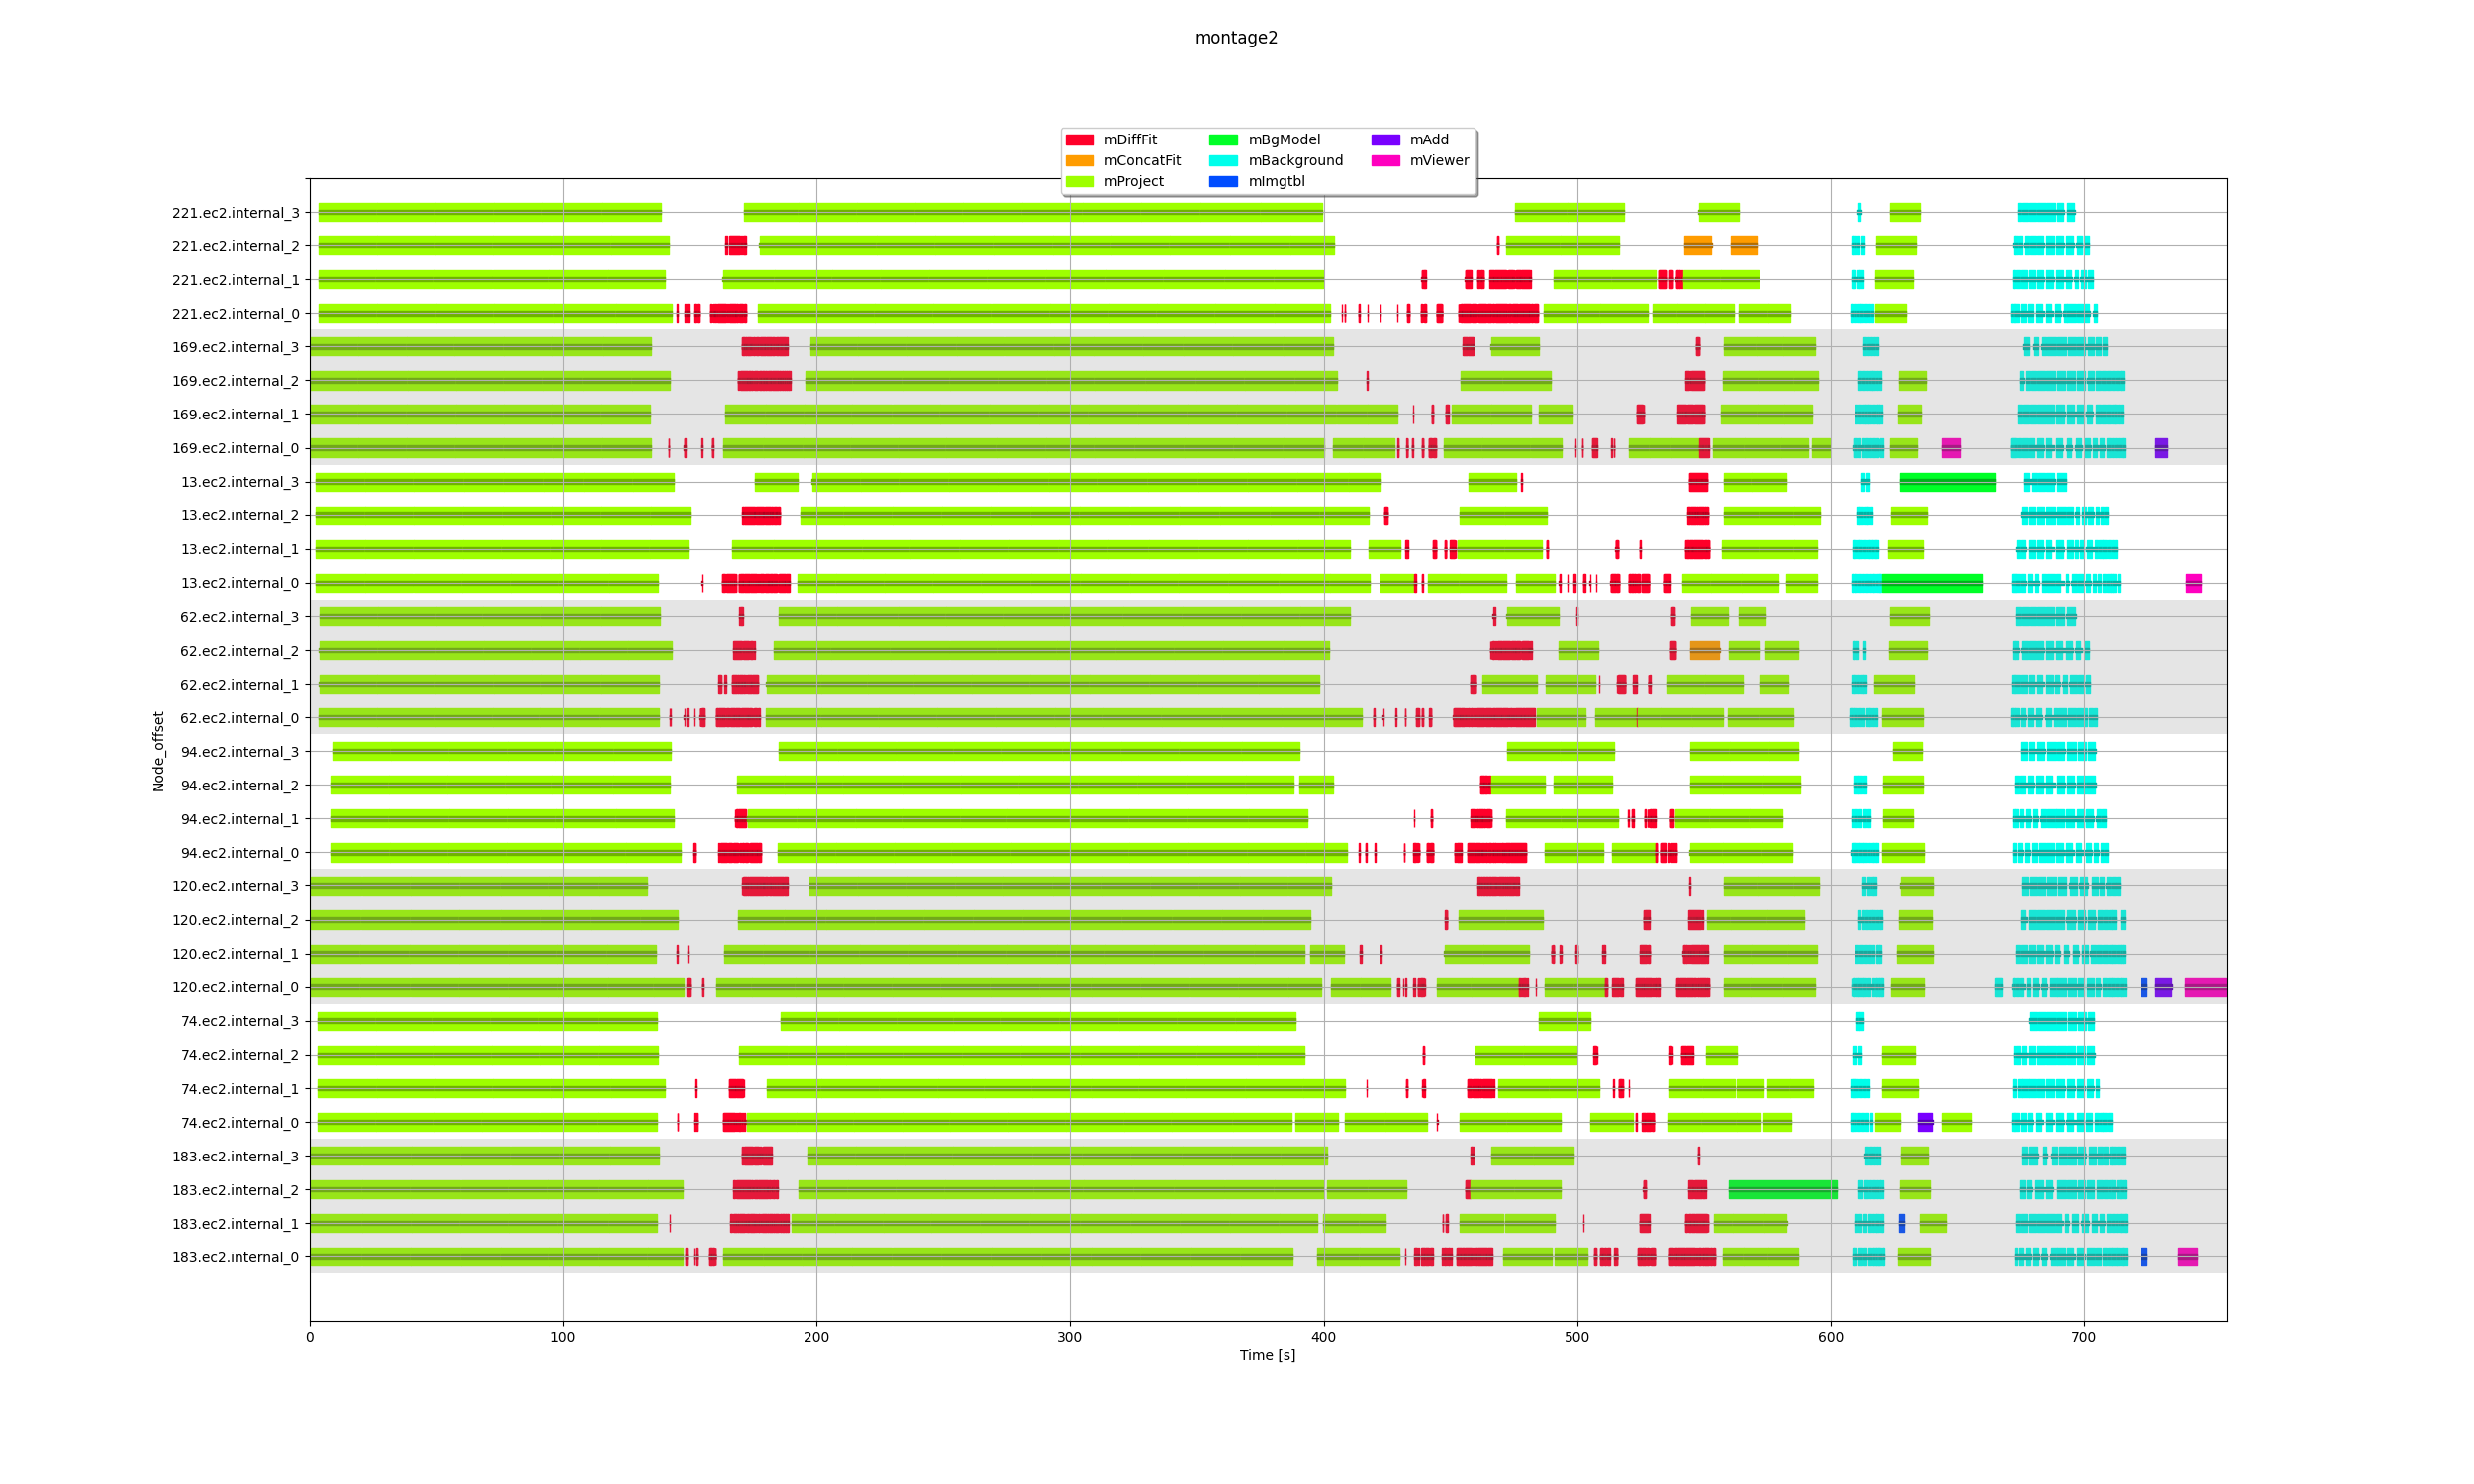
\includegraphics[width=1\linewidth]{figures/6-2-m1.0-agglo-peft.png}
% \caption[Task clustering on PEFT-planned schedule - Montage-1.0]{Task clustering on PEFT-planned schedule - Montage-1.0.}
% \label{fig:evaluation:agglo:m10:peft}
% \end{figure}
%%%%


